% ======================================================================= %
%            Bi-directional dual arm object handover
% ======================================================================= %
	
{\color{blue}\chapter{Proactive whole-body object handover}\label{handover chapter}}


In previous human-robot interaction studies~\cite{huber2008human, strabala2013toward, shibata1995experimental} and also in our work in Chapter~\ref{more than just co-workers}, we have shown that the human acceptance of the robot co-worker during a task increases when both the appearance and behaviour (motion) of the robot are similar to that of humans; especially during an interactive task. In this study, we also use HRP-2Kai as the robot co-worker.

We discussed our findings in \textit{non-physical} human-robot interaction. Here we introduced a framework particularly focused on intuitive and proactive bi-directional object handover between a human-humanoid dyad using Whole-Body Control (WBC). This study concerns \textit{physical} human-robot interaction (pHRI). We enhance our whole-body motion controller~\cite{bouyarmane2018quadratic} with tasks to achieve bi-directional object handover between human and humanoid robot co-workers. We took inspiration and insights from existing state-of-the-art works in object handover between human-human and human-robot dyads and extended some ideas to bi-manual and locomotion synchronized handovers.


\section{Handover routine}\label{handover routine}

We take similar approach as~\cite{medina2016human, nemlekarprompt} and treat the continuous process of object handover between human and humanoid as \textit{sequence}, such that object handover from human to humanoid is one \textit{sequence} and return of object to human is another \textit {sequence}. These two handover \textit {sequence}s make one handover \textit{routine}. An overview of handover \textit{sequence} is illustrated in (Fig.~\ref{fig:handover routine}).


\begin{figure}[htbp]
	\centering{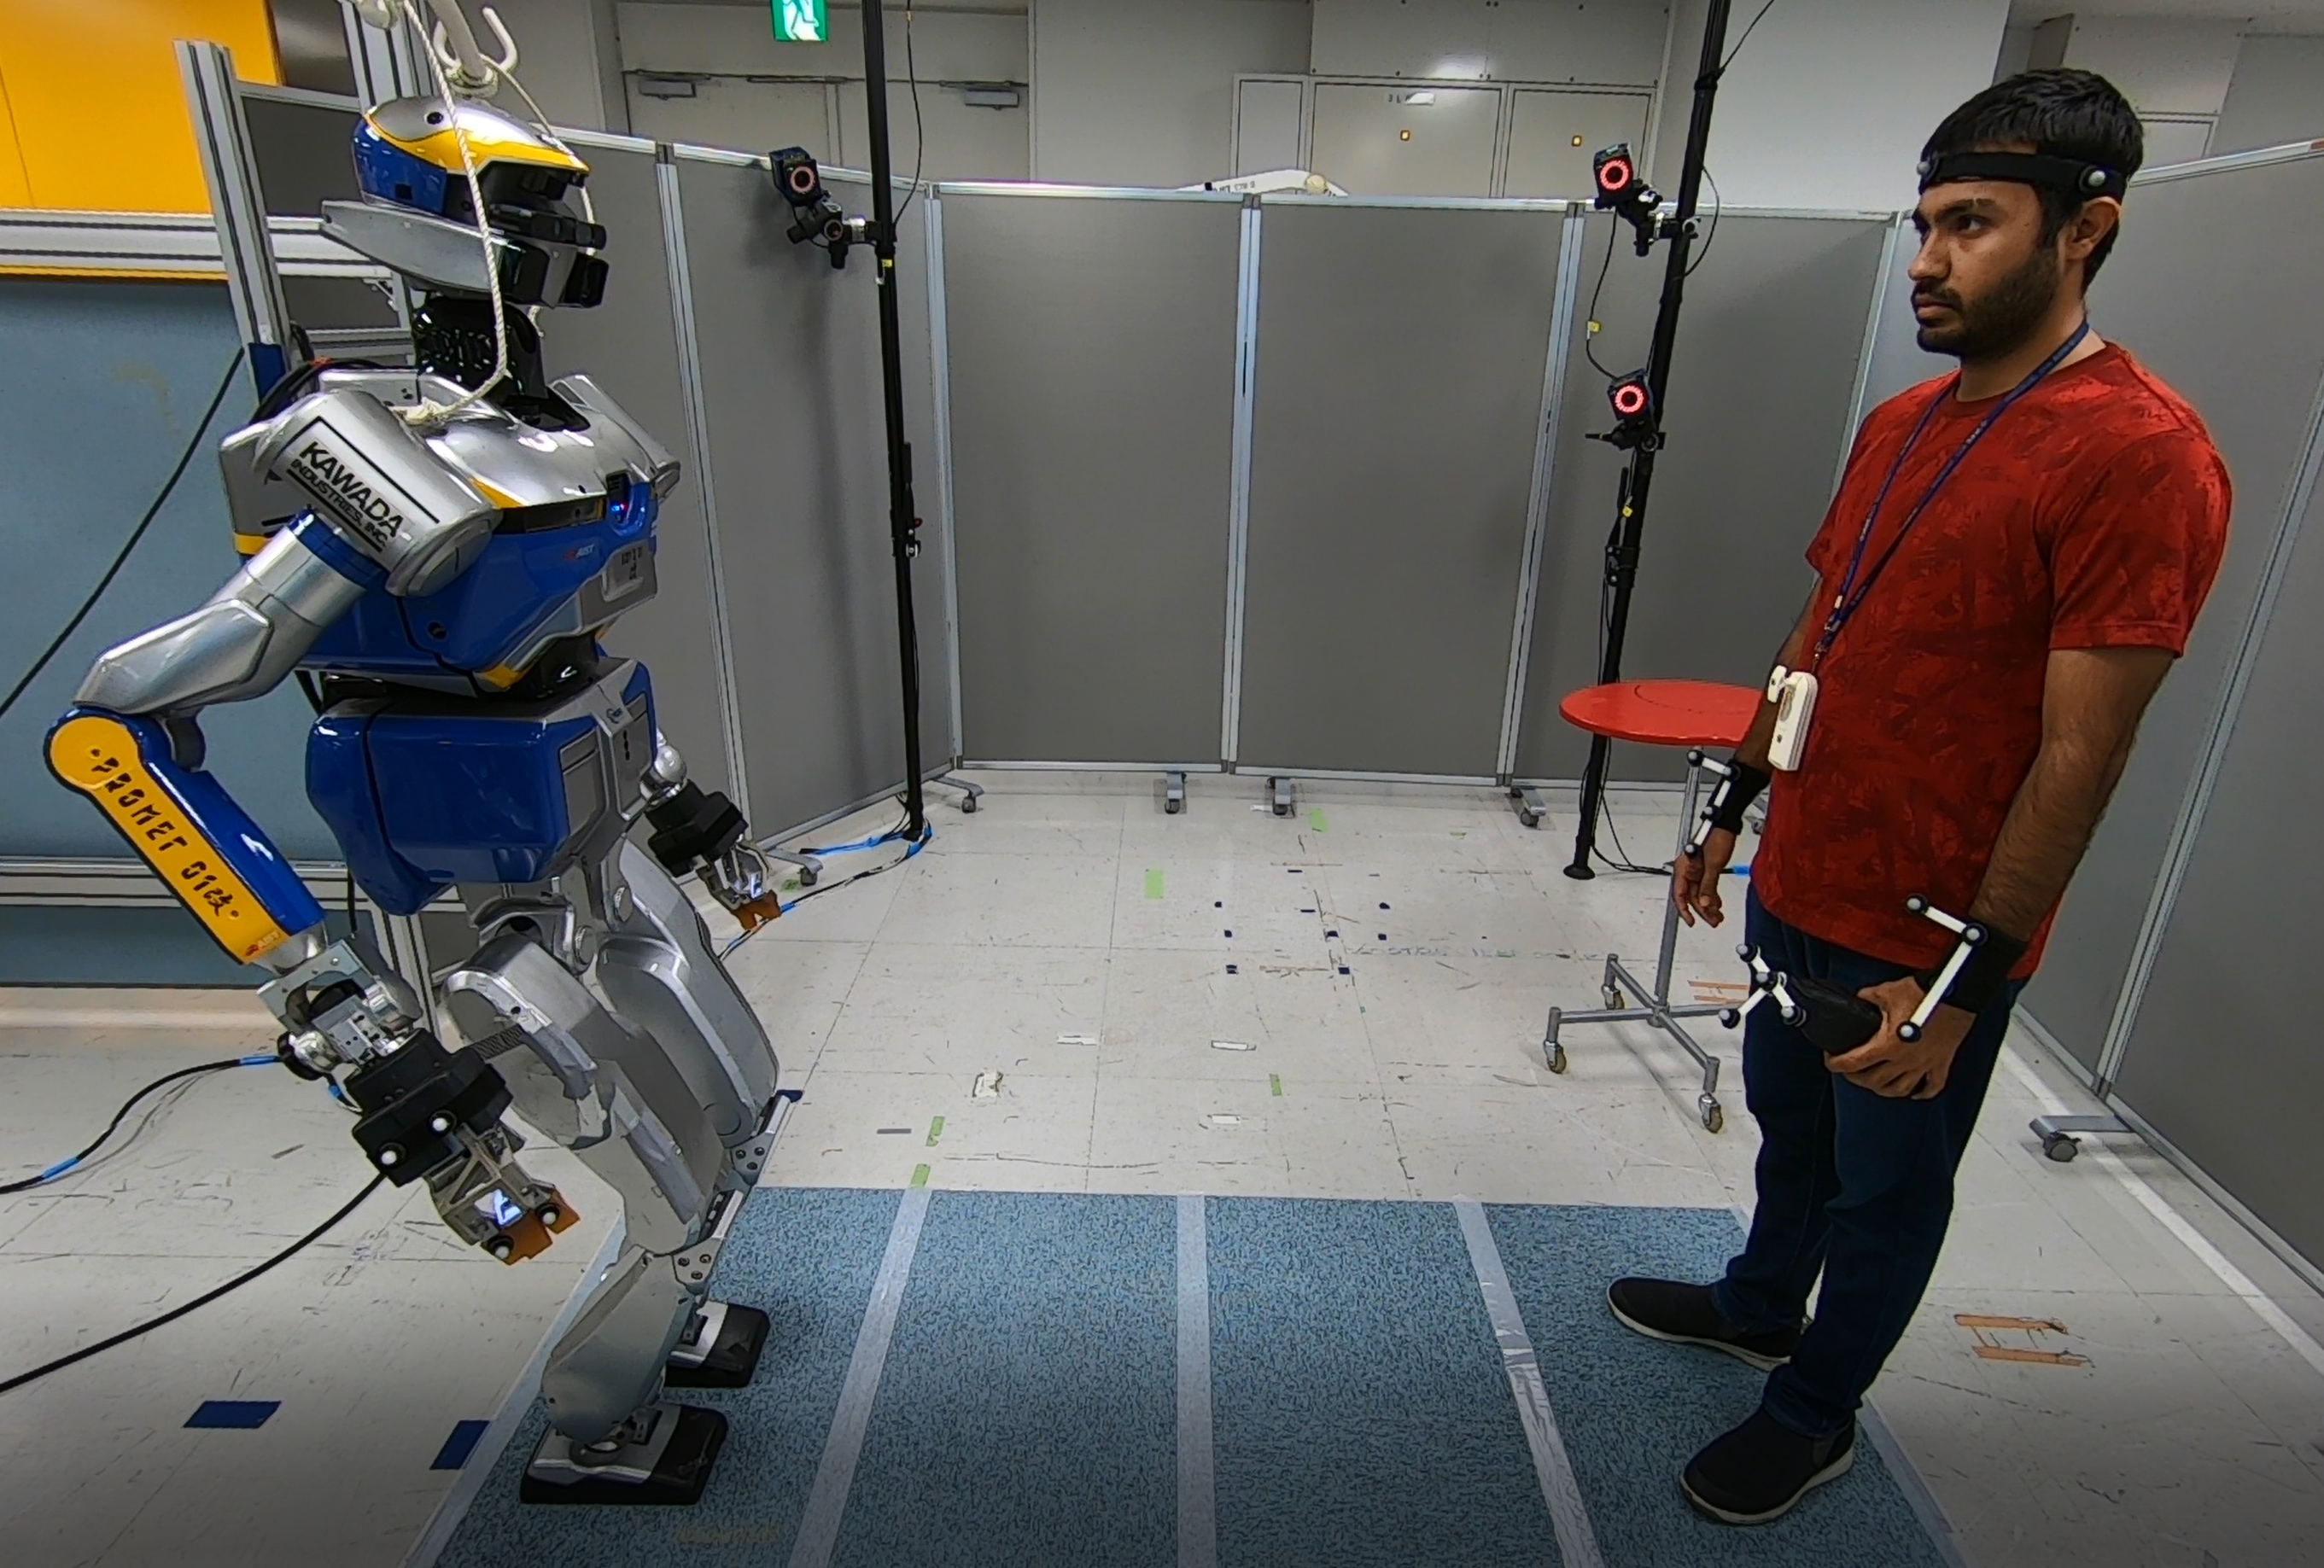
\includegraphics[width=0.8\columnwidth]{plots/c4-plots/halfsit}}
	\caption{Human and humanoid starting posture.}
	\label{fig:halfsit}
\end{figure}


Within the handover routine, both human and robot always start from a standing posture (see Fig.~\ref{fig:halfsit}). The robot standing posture has a Center of Mass CoM(z) height $0.87$ meters. We assume that human is ready with the intention to handover the object if he/she is holding the object in his/her hand. The only predefined condition is that human must seriously exchange the object with a robot in one continuous shot. The human can choose his/her hand configuration, speed, trajectory and the handover location but within the robot's reachable workspace.

During 1$^\text{st}$ \textit{sequence} of handover \textit{routine}, the human carries the object to different handover locations with distinguishable orientations of the object carrying hand and tries to give the object to the robot. Similarly, during 2$^\text{nd}$ \textit{sequence} of handover, human approaches somewhere in the robot reachable workspace to receive the object from robot using his/her choice of hand orientation and preferred handover location. The robot end-effectors reachable workspace is given by equation (\ref{reachable}), object handover can occur as long as estimated handover location is within this region.

\begin{equation}\label{reachable}
\centering
1 = 
\begin{cases}
X_{\min} <= {}^{h}\mathcal{P}_{\text{ef}}(x) <= X_{\max} \quad  \\
Y_{\min} < {}^{h}\mathcal{P}_{\text{ef}}(y) <= Y_{\max} \quad  \\
{}^{h}\mathcal{P}_{\text{ef}}(z) >= CoM(z)

\end{cases}
\end{equation}

where, $ {}^{h}\mathcal{P}_{\text{ef}} $ is the relative 3D position of active human hand \texttt{w.r.t} robot end-effector. The default values of $ X_{\min} $ and $ X_{\max} $ are $ 0.1 $ and $ 0.8 $ meters respectively, for robot left end-effector $ Y_{\min} $ and $ Y_{\max} $ are $ 0.15 $ and $ 0.75 $ meters respectively, while for robot right end-effector $ Y_{\min} $ and $ Y_{\max} $ are $ -0.75 $ and $ 0.15 $ meters respectively.

Just like during human-human object handover, another thing that we incorporated in our handover \textit{routine} is to give visual tracking like behaviour to HRP-2Kai by following an object or active human hand using robot's head, depending on the handover \textit{sequence}. Using a \texttt{gaze} task (\nameref{QPTasks}), HRP-2Kai follows object during 1$^\text{st}$ \textit{sequence} of handover and follows active human hand which is approaching to retrieve the object during 2$^\text{nd}$ \textit{sequence}.

Hereafter and until section (\nameref{both hands individual}) we will formulate the handover \textit{routine} using human right hand and robot left end-effector; afterwards we will generalize our one-handed handover \textit{routine} for four possible handover combination scenarios:

\begin{itemize}
	\item \textbf{human right hand $\longleftrightarrow$ robot left end-effector}
	\item human left hand $\longleftrightarrow$ robot left end-effector 
	\item human left hand $\longleftrightarrow$  robot right end-effector
	\item human right hand $\longleftrightarrow$ robot right end-effector
\end{itemize}


\begin{figure}[pt]
	\centering
	\tikzstyle{line} = [draw, -latex']
	
	\tikzstyle{cloud} = [draw, ellipse,fill=blue!20, text width=6em, text centered, node distance=4cm,  inner sep=0pt, minimum height=2em]
	
	\tikzstyle{startstop} = [rectangle, text centered, rounded corners, minimum width=3cm, minimum height=1cm, draw=black, node distance=4cm, fill=red!30]
	
	\tikzstyle{io} = [trapezium, trapezium left angle=70, trapezium right angle=-70,text centered, text width = 1cm,minimum height=1cm, minimum width=2cm, node distance=4cm, draw=black, fill=red!30]
	
	\tikzstyle{process} = [rectangle, text centered, minimum width=1cm, minimum height=1cm, draw=black, fill=orange!30]
	
	\tikzstyle{block} = [rectangle, draw, fill=green!20, text width=10em, text centered, node distance=4cm, minimum height=4em]
	
	\tikzstyle{decision} = [diamond, draw, fill=yellow!20, text width=6em, text badly centered, node distance=4cm, inner sep=0pt]
	
	\begin{tikzpicture}[node distance = 3cm, auto]
	
	\node [process] (or) {1$^\text{st}$ or 2$^\text{st}$ \textit{sequence}};
	
	\node [startstop, above of=or, node distance = 2cm, auto] (start) {start handover routine};	
	
%	\node [cloud, left of=or] (subj) {human has object};
%	\node [cloud, right of=or] (robot) {robot has object};
	
	\node [block, below of=or, node distance=2cm] (init) {initialize prediction model};
	\node [io, right of=init] (in1) {robot Ef pose};
	\node [io, left of=init] (in2) {human hand pose};
	
	\node [block, below of=init, node distance = 3cm, auto] (relativePos) {observe and track active human hand pose relative to robot Ef pose};
	
	\node [decision, below of=relativePos] (within) {has human hand arrived within robot's reachable workspace?};
	
%	\node [block, left of=within, node distance=5cm, text width=5em] (wait) {wait \& head-track human hand};
	
	\node [decision, right of=within, node distance=5cm, text width=5em] (walk) {did human moved backward?};
	
	\node [block, below of=walk, node distance=3cm, text width=5em] (trigger) {trigger walk};
	
	\node [block, below of=within, node distance=4cm] (moveEf) {start moving robot Ef to predicted position};
	
	\node [decision, below of=moveEf, node distance = 4cm] (ifClose) {is human hand close enough to robot?};
	
	\node [block, right of=ifClose, node distance = 5.5cm] (keep moving) {keep moving Ef towards predicted position};
	
	
	\node [startstop, below of=ifClose, node distance=3cm] (event) {handover object};
	
	% Draw edges
%	\path [line] (subj) -- (or);
%	\path [line] (robot) -- (or);
	\path [line] (start) -- (or);
	\path [line] (or) -- (init);
	
	\path [line,dashed] (in1) -- (init);
	\path [line,dashed] (in2) -- (init);
	\path [line] (init) --  node {FSM} (relativePos);
	\path [line] (relativePos) -- (within);
	
%	\path [line] (wait) |- (relativePos);
%	\path [line] (within) -- node [near start] {no} (wait);
	\path [line] (within) -- node {yes} (moveEf);
	
	\path [line] (within) -- node [near start] {no} (walk);
	\path [line] (walk) -- node [near start] {yes} (trigger);
	\path [line] (walk) |- node [near start] {no} (relativePos);
	
	\path[line] (moveEf) -- (ifClose);
	\path [line] (ifClose) -- node [near start] {no} (keep moving);
	\path [line] (ifClose) -- node [near start] {yes} (event);
	
	\end{tikzpicture}
	
	\caption{General overview of human humanoid handover \textit{sequence}. 1$^\text{st}$ (human has object) or 2$^\text{nd}$ (robot has object).}
	\label{fig:handover routine}
\end{figure}


\section{Experimental setup}

Our experiment setup is shown in (Fig.~\ref{fig:halfsit}). Initially, we started by having a human co-worker and robot co-worker standing comfortably in front of each other at a distance of $1.2$ meters from each other. This distance is known to be the social distance in human proxemics~\cite{hall1966proxemic}. Movable panels partially enclosed the whole setup.

\subsection{Robot}

We used an HRP-2Kai robot~\cite{Kaneko:RAS_ICHR:2015} as the co-worker. The human and humanoid are free to use their both hands, end-effectors respectively in handing over the objects.

\subsection{Mocap}

We used motion capture (in short \textit{mocap}) system manufactured by ({\it Motion Analysis Co.,}), to track and get the position data of the passive reflective markers. We used twenty passive reflective markers in several handover scenarios. We placed four markers on each end-effectors, three markers were placed on the head of the human co-worker to get his/her position in mocap frame, three markers were placed on each of the hands of a human co-worker and also on the object itself. The markers on the human hands and object were utilized to get their respective position, and orientation in the mocap frame and we used makers on the robot end-effectors during object handover and release-return of object from the robot grippers to human co-worker as a substitute to lack of haptic feedback, see section (\nameref{interaction model}) for more details. These passive markers were tracked using ten kestrel infra-red cameras, each at 200 Hz. These mocap markers position data was utilized using a real-time interface between mocap system (\texttt{cortex}) and \texttt{ROS} called \textit{ros-cortex-bridge}, which was designed to transmit this position data to the robot controller in real-time.

\subsection{Handover object(s)}

As shown in (Fig.~\ref{fig:objects}), we used three easily distinguishable objects during the one-handed handover between the human-humanoid dyad. The mass of objects varies from $0.22$ kg to $1.1$ kg.


\begin{figure}[H]
	\centering{\includegraphics[width=0.4\columnwidth]{plots/c4-plots/objects}}
	\caption{Distinguishable shape and mass objects used during one-handed handover between human and humanoid co-worker.}
	\label{fig:objects}
\end{figure}

\section{Robot QP controller}\label{QPController}

We used our research group's native multi-objective Quadratic Programming (QP)~\cite{ladder-HRP-2Kai} based low-level Whole-Body Control (WBC) to govern and optimize the motion of HRP-2Kai. ``WBC exploits the full potential of the entire floating based robot body and allows interaction with the environment using multi-contact strategies''. It also allows concurrent execution of several tasks at once, for example using WBC, the humanoid can utilize one or both of its end-effector(s) to grasp and manipulate the object while at the same time takes a step forward or backward, allowing itself to reach the handover location. 

To realize human, humanoid bi-directional object/tool handover, we introduced several tasks and formulated them in a quadratic fashion, so it conforms with QP based controller. The QP enables whole-body control of our HRP2-Kai while respecting both internal and external constraints. Few such constraints encompass joints limits, force and torque limits, contact constraints, stability constraints such as keeping the centre of mass (CoM) inside the support polygon along with self-collision constraints with the environment and itself while generating optimal joint trajectories. Below we mentioned some significant constraints that a robot must satisfy at each time step during human-robot object handover.


\subsection{QP constraints}\label{QPConstraints}

The QP controller's objective is to compute an acceleration of $\ddot{q}$, where $q$ is the robot configuration vector at each time step ($dt$)  to achieve a set of targets or tasks. At each $dt$, the QP is formulated and solved by the LSSOL solver~\cite{gill1986fortran}. The tasks are formulated either linear constraints or quadratic costs~\cite{ladder-HRP-2Kai}. However, we want to solve these tasks in a best possible manner as a linearization of some tasks may not be feasible or maybe conflicting, therefore using least-square approximation, the quadratic cost $c$ corresponding to a task $\mathscr{T}_i =0$ is given by:


\begin{equation}
c_i(q,\dot{q}, \ddot{q})  = \frac{1}{2}{\norm{ J_i\ddot{q} + \dot{J}_i\dot{q} -\ddot{\mathscr{T}}_i }^2 }
\end{equation}

where $J_i$ the Jacobian matrix of $\mathscr{T}_i$, and the quadratic objective function of QP controller would be,

\begin{equation}\label{qp equation}
\min_{\ddot{q},\tau,f} \; \sum_{i\in O} \omega_i c_i(q,\dot{q},\ddot{q}) + \omega_{f}\lVert f\rVert^2
\end{equation}

which is subject to constraint on equation of motion, as well as other below mentioned constraints,

\begin{equation}
	M(q)\ddot{q} + N(q,\dot{q}) =  J_c^T f
\end{equation}

where $f$ is the set of contact forces, $M$ denotes the inertial matrix of the robot, $N$ accounts for Coriolis and gravity effects, $J_c$ is the Jacobian matrix of all points of contact. 

The QP objective function in equation (\ref{qp equation}) is made of two terms and the tasks $\mathscr{T}_i$ mentioned in next subsection (\nameref{QPTasks}) are weighted against each other by weight $w_i$ based on their relative importance and priority. While the damping weight $w_f$ ensures the smoothness and uniqueness of solution by keeping Hessian matrix positive definite.

\begin{enumerate}	
	\item Static equilibrium:

	$\underline{\tau} \leq J^i(q_i)^Tf_i - g^i(q_i) \leq \overline{\tau}$
	
	where sub-script or super-script $i$ is the $i$-th robot, $q_i$ is the $i$-th robot configuration vector, $f_i$ is the set of contact forces vector of $i$-th robot, $J$ is the Jacobian matrix of all points of contact forces, and $\overline{\tau}$ and $\underline{\tau}$ are the maximum and minimum steady state torque limits respectively, and g be the gravity constant.
	
	\item Joint limits:
	
	$\underline{q_i} \leq q_i \leq \overline{q_i}$
	
	$\underline{q_i}$ and $\overline{q_i}$ are the lower and upper limits for robot joints.
	
	\item Self collisions:
	
	$\delta(X^i_j(q_i), X^i_k(q_i)) > \epsilon_{jk} \qquad \forall(j,k)\in {\mathscr{I}}^i_{\text{self\;collision}}$

	$\delta$ is the function of distance, $X^i_j(q_i)$ is the occupied volume by $j$-th body of robot in configuration $q_i$, $\epsilon_{jk}$ is the pair of user select minimum distances ($j$,$k$) and ${\mathscr{I}}^i_{\text{self\;collision}}$ is the robot sets of self collision pairs.
	
	\item Environment collision:
	
	$\delta(X^i_j(q_i), X_k) > \epsilon_{jk} \qquad \forall(j,k)\in {\mathscr{I}}^i_{\text{robot\;environment}}$
	
	${\mathscr{I}}^i_{\text{robot\;environment}}$ is the set of robot environment (object) collision pairs.
	
	\item Contact Constraint: $\mathscr{I}_\text{contact} = J_i(q) (\dot{q}_{s(k)} - \dot{q}_{p(k)}) = 0$\\
	The objective of this constraint is to maintain a null velocity~\cite{ohwovoriole1980externsion} between the joints of bodies in contact, where $p(k)$ and $s(k)$ are the predecessor and successor bodies of a robot(s) in contact that imposes a constraint~\cite{featherstone2014rigid}.
\end{enumerate}

%%%	\item acceleration Constraint: $\mathscr{I}_{contact} = J_i(q)\ddot{q}_{s(k)} + \dot{J}(q)_i\dot{q}_{p(k)} = 0$\\


\subsection{QP tasks}\label{QPTasks}

As mentioned earlier, below, we introduced the following outlined tasks to the multi-objective QP controller to achieve safe and reliable human-robot object handover. Let function $\mathscr{T}_i(q)$ denote the geometric objectives (task error) that we require to regulate to zero or maintain above zero, i.e. $\mathscr{T}_i(q) = 0$ and $\mathscr{T}_i(q) \geq 0$.  

\begin{enumerate}[start=1,label={\arabic*.}]

\item Posture task: $\mathscr{T}_\text{posture} = q_d - q = 0$\\
Posture task is the first task that is added to the QP controller, it allows the robot to maintain an initial posture.

\item Com task: $\mathscr{T}_\text{CoM} = \text{CoM}_d - \text{CoM}(q) = 0$\\
Com task is used in conjunction with the stability constraint to all time maintain the CoM position inside the support polygon. 

\item Joint limit task: $\mathscr{T}_\text{jlim} = \underline{q_i} \leq q_i \leq \overline{q_i}$\\
This task is used occasionally whenever there is a need to limit certain joint movements.  

\item Position task at body $k$: $\mathscr{T}_\text{pos} = r^d_k - r_k(q) = 0$\\
Where, $r_k$ and $r^d_k$ are the current and desired position of $i$-th robot $k$-th body. Robot end-effector position task is used to reach the desired handover location~\cite{ladder-HRP-2Kai}.

\item Orientation task at body $k$: $\mathscr{T}_\text{ori} = Err((E^d_k),  E_k(q))$\\
Where, $E_k$ is the orientation of $i$-th robot body to world. Robot end-effector orientation task is used to compute orientation relative to human hand orientation.

\item Gaze task : $\mathscr{T}_\text{gaze} =u_\text{target} - u = 0$\\
Where, $u_\text{target}$  and $u$ are the target vector in world and body vector that needs to be oriented respectively. We used gaze task to orient the head joints of HRP-2Kai towards the active human hand position in the world; more details can be found in~\cite{samy2017VecOriTask}. Note that by active human hand we meant by either object carrying human hand during human-to-robot handover trial or by the hand which is approaching to grasp the object during robot-to-human handover trial.

\end{enumerate}


%\clearpage

\section{Notations}

Let $\mathcal{M}$ (Mocap) and $\mathcal{R}$ (Robot) be the two fixed frames with the same orientation that represent both Cartesian coordinate systems and Pl\"ucker coordinate systems denoted by $X$ in the Euclidean space. Both $\mathcal{M}$ and $\mathcal{R}$ are defined by their position and orientation of a Cartesian frame, such that ${}^MX_R$ denotes the Pl\"ucker coordinate transform which depends only on the position and orientation of frame $\mathcal{M}$ relative to frame $\mathcal{R}$ (see Fig~\ref{fig:frames}).

\begin{figure}[ht]
	\centering{\includegraphics[width=0.5\columnwidth]{plots/c4-plots/frame}}
	\caption{$\mathcal{M}$ and $\mathcal{R}$ Cartesian coordinate systems.}
	\label{fig:frames}
\end{figure}


\begin{itemize}	
	\item  We used 6D spatial vectors to express the pose of human hands and robot end-effectors as well as objects. We, therefore, adopt a 6D notation based on spatial vectors, which was explained in Chapter 2 of~\cite{featherstone2014rigid}.
		
	\item One can receive and control the robot end-effector current orientation ${{}^{\text{ef}}\mathcal{O}_R} \in \mathbb{R}^{3\times3}$ and current position ${{}^{\text{ef}}\mathcal{P}_R} \in \mathbb{R}^{3}$ respectively in the $\mathcal{R}$ frame, by using QP's \texttt{Orientation} task and \texttt{Position} task (see subsection~\nameref{QPTasks}), therefore,
	\begin{gather}\label{X_R_ef}
	{}^{\text{ef}}{X}_R =
	\left[\begin{array}{cc}
	{}^{\text{ef}}\mathcal{O}_R & {}^{\text{ef}}\mathcal{P}_R
	\end{array}\right]
	\end{gather}
	
	\item Likewise, ${{}^{h}\mathcal{O}_M} \in \mathbb{R}^{3\times3}$ and ${{}^{h}\mathcal{P}_M} \in \mathbb{R}^{3}$, denotes the human hand $h$ orientation and position respectively in the $\mathcal{M}$ frame, obtained from the ${\bf L}$ shape body (see Fig.~\ref{fig:lshapes}), which is later further explained in section (\nameref{orientation_model}),
	\begin{gather}\label{X_M_h}
	{}^{h}{X}_M =
	\left[\begin{array}{cc}
	{}^{h}\mathcal{O}_M & {}^{h}\mathcal{P}_M \\
	\end{array}\right]
	\end{gather}
	
	\item ${{}^{h}\mathcal{O}_{\text{ef}}} \in \mathbb{R}^{3\times3}$ and ${{}^{h}\mathcal{P}_{\text{ef}}} \in \mathbb{R}^{3}$ respectively, denotes the human hand $h$ orientation and position relative to robot end-effector,
	\begin{gather}\label{X_ef_h}
	{}^{h}{X}_{\text{ef}} =
	\left[\begin{array}{cc}
	{}^{h}\mathcal{O}_{\text{ef}} & {}^{h}\mathcal{P}_{\text{ef}} \\
	\end{array}\right]
	\end{gather}
	
	\item Let ${{}^{o}\mathcal{O}_M} \in \mathbb{R}^{3\times3}$ and ${{}^{o}\mathcal{P}_M} \in \mathbb{R}^{3}$, denotes the object orientation and position respectively in the $\mathcal{M}$ frame, obtained from another ${\bf L}$ shape body (see Fig.~\ref{fig:lshapes}) attached on the object.
	\begin{gather}\label{X_M_o}
	{}^{o}{X}_M =
	\left[\begin{array}{cc}
	{}^{o}\mathcal{O}_M & {}^{o}\mathcal{P}_M \\
	\end{array}\right]
	\end{gather}
	
	\item For convenience, we formulated the problem with a common origin {\it O}, such that $\mathcal R \equiv M$ (both frames are located between the feet of robot HRP-2Kai), therefore, we can get human hand pose \texttt{w.r.t.} or relative to robot end-effector
	\begin{equation}\label{X_ef_h1}
	{}^{h}{X}_{\text{ef}} = {}^{h}{X}_{M}  {}^{\text{ef}}{X_{R}}^{-1}
	\end{equation}
	\item otherwise, when $\mathcal R \neq M$, using Pl\"ucker transform ${}^MX_R$,
	
	\begin{equation}\label{X_ef_h2}
	{}^{h}{X}_{\text{ef}} = {}^{h}{X}_{M}  {\bf{}^{M}{X}_R}  {}^{\text{ef}}{X_{R}}^{-1}
	\end{equation}

\end{itemize}


\begin{figure}[htpb]
	\centering{\includegraphics[width=.9\columnwidth]{plots/c4-plots/lshpe-lt-rt}}
	\caption{${\bf L}$ shape rigid body on the human hand(s)}
	\label{fig:lshapes}
\end{figure}

Note that, the mathematical notations in the following sections follow ISO guidelines. The Euclidean distance is represented in meters. The time unit is set in seconds or mentioned otherwise.


\section{Position prediction model}\label{prediction_model}

In case of object handover and when the human co-worker is ready with the intention to handover the object, instead of merely waiting for the object to be presented by the human at the handover location, the robot must proactively plan its own movements by observing past and predicting near-future human hand movements so that it could arrive at the human chosen handover location approximately at same time ---either to receive or return the object. Therefore, the estimation of handover time, as well as the approximation of handover location, must be realized early during the handover \textit{sequence}. Note that this proactive nature of the robot co-worker should also be available when the human co-worker requests for the object.

Here we designed a prediction model, with robot left end-effector pose $\mathcal{}^{\text{ef}}{X}_R$ (\ref{X_R_ef}) and human hand mocap marker position ${}^{h}\mathcal{P}_M$ (\ref{X_M_h}) as inputs. Note that for simplicity, we formulated the problem with a common origin {\it O}, such that frame $\mathcal R \equiv M$. To get the position and orientation of the human hand, we placed a rigid body with a shape similar to an alphabet ${\bf L}$ on the wrist of a human hand(s) and on the object as shown in (Fig.~\ref{fig:lshapes}). The three mocap markers $A, B$ and $C$ make up the three vertices of ${\bf L}$ shape body. Note that from onward by ${}^{h}\mathcal{P}_M$ we would mean the position of point $A$ on the ${\bf L}$ shape body as the human hand marker position (Fig.~\ref{fig:lshapes}).

The prediction model behaviour can be tuned by two initially required constant sample size, $i_\text{observe}$ ---a predefined sample size required to observe the motion of the human hand and $i_\text{predict}$ ---required to predict the human hand position in advance.

In order for the handover between human and humanoid to be smooth and intuitive, the robot needs to proactively estimate the near future position of human hand in advance, during both \textit{sequence}s when robot act as receiver (1$^\text{st}$ \textit{sequence}) or when robot acts as giver (2$^\text{nd}$ \textit{sequence}) of a handover \textit{routine}. Therefore we formulate the movements of the human hand as a constant velocity based linear motion model to predict his/her hand (hence handover) position continuously. The robot observes human hand movements for a predefined sample size $i_\text{observe}$ along with the average velocity of his/her hand during that time and then predicts the near future human hand movement direction and position using equations (\ref{predictVel}) and (\ref{predict}) for the predefined  $i_\text{predict}$ sample size.

\begin{equation} \label{predictVel}
{}^{h}\mathcal{\bar{V}}_{M} = \frac{1}{i_\text{observe}}{\sum_{j=1}^{j=i_\text{observe}} ({}^{h}\mathcal{P}_{M}(j)-{}^{h}\mathcal{P}_{M}(j-1))/dt }
\end{equation}

\begin{equation} \label{predict}
{}^{h}\mathcal{P}_M(i_\text{predict}) = {}^{h}\mathcal{\bar{V}}_{M} \cdot (i_\text{predict}  - i_\text{observe})  \cdot dt + {}^{h}\mathcal{P}_{M}(i_\text{observe})
\end{equation}


where $dt$ is controller run-time, in our case it is 5ms as mentioned earlier in the section (\nameref{QPController}). $j$ in equation (\ref{predictVel}) is sample index. ${}^{h}\mathcal{\bar{V}}_{M}$ is the average human hand movement velocity during $i_\text{observe}$ sample size. ${}^{h}\mathcal{P}_M(i_\text{predict})$ is the predicted position of human hand at $i_\text{predict}$. The prediction model updates and converges itself over time and in doing so updates the robot end-effector position towards the active human hand, upon condition if predicted position is within the robot end-effector's reachable workspace. 

Recalling equation (\ref{X_ef_h1}) or (\ref{X_ef_h2}), the updated translation component of pl\"ucker transformation ${}^{h}{X}_{\text{ef}}$, which provides the predicted position of human hand with respect to robot end-effector in the robot coordinate system is given by (\ref{X_ef_ht}).

\begin{equation}\label{X_ef_ht}
{}^{h}{X}_{\text{ef}}(i_\text{predict}) =  {}^{h}{X}_M  {}^{M}{X}_R {{}^{\text{ef}}{X}_R}^{-1}
\end{equation}

where, ${}^{M}{X}_R$ is the Pl\"ucker coordinate transform frame $\mathcal{M}$ relative to frame $\mathcal{R}$, if $\mathcal R \neq M$.


Finally, the handover location is estimated based on the human hand predicted position when the following conditions satisfy (\ref{min_posErr_vel}), that is when the human hand velocity is minimum and robot end-effector is closest to the human hand.

\begin{equation}\label{min_posErr_vel}
\begin{cases}
	\norm{{}^{h}\mathcal{\bar{V}}_{M}}& <= 1e^{-2} \\
	\norm{({}^{h}\mathcal{P}_{M}(i_\text{predict}) - {}^{\text{ef}}\mathcal{P}_{R})} & <= 2e^{-2}
\end{cases}
\end{equation}

where, ${}^{h}\mathcal{P}_{M}(i_\text{predict})$ is the desired position for robot end-effector to reach and ${}^{\text{ef}}\mathcal{P}_{R}$ is the actual current position of robot end-effector and also both positions are in same frame or transformed otherwise. We have also explained the procedure of predicting human hand position and estimating handover location in Algorithm (\ref{positionalgo}) of (\nameref{handoverAppendix}).

In this section, we presented how to predict and estimate the handover location, though just by knowing the handover location in space is not enough for an optimal smooth handover of an object. Therefore in next section (\nameref{orientation_model}), we will present the orientation component of ${}^{h}{X}_{\text{ef}}$ which gives the graspable relative orientation of robot end-effector \texttt{w.r.t} human hand or object orientation during handover.


\section{Grasp configuration model}\label{orientation_model}

To take into account comfort and requirement of the human co-worker, it is pivotal for the robot to be able to find the most appropriate configuration to grasp (as \textit{receiver}) or release (as \textit{giver}) the object~\cite{cakmak2011human, aleotti2012comfortable}. Therefore for an intuitive and smooth handover of an object, the robot should relatively orient it's end-effector and configure according to the orientation of either object (1$^\text{st}$ \textit{sequence}) or human hand (2$^\text{nd}$ \textit{sequence}) during the handover \textit{routine}. Though there are several possible configurations to handover an object, the robot must determine the correct configuration of its end-effector during the handover which is suitable and comfortable enough for the human and could be perceived natural in the eyes of a human co-worker. Note that in this study, we mainly chose to handover the object in which it is most commonly being grasped (default configuration) hence natural to the eyes of the human, one example would be holding an object such as a water bottle when its cap is in the upright position during the handover. 

We propose a simple method to get the desired object grasping orientation of robot end-effector either by considering the relative orientation of the active human hand or the object itself. This handover grasp configuration model consists of two sub-models, in first sub-model, we determine the orientation of the active human hand or object itself. In the second sub-model, we utilize the first sub-model to continuously get the desired relative orientation of the robot end-effector during the handover \textit{routine}. 


%%% 1st sub-model

To determine the object or active human hand orientation, as  mentioned in previous section we placed an ${\bf L}$ shape rigid body on the wrist of the human hand(s) and a similar one on the object as well such that during the object handover scenario, vector $\vec{AB}^{\,}$ along the longer side and vector $\vec{BC}^{\,}$ along the shorter side of the ${\bf L}$ shape are set to be parallel with the $X$-axis and $Y$-axis of the mocap frame $\mathcal{M}$ respectively, as well as orthogonal to each other (as shown in Fig.~\ref{fig:lshapes}). For simplicity, let us consider $\hat{x}$ be the unit vector, which is parallel and along the $X$-axis and likewise a unit vector $\hat{y}$ is parallel and along the $Y$-axis of the mocap frame $\mathcal{M}$, such that

\begin{equation*}
\hat{x} = \frac{\vec{AB}^{\,}}{\norm{\vec{AB}^{\,}}}
\end{equation*}

\begin{equation*}
\hat{y} = \frac{\vec{BC}^{\,}}{\norm{\vec{BC}^{\,}}}
\end{equation*}

Let ${}^{h}\mathcal{O}_{M}$ in equation (\ref{X_M_h}) be the rotation matrix representing the orientation of human hand (or object) in the mocap frame $\mathcal{M}$ and since $\hat{x} \in \mathbb{R}^{3}$ and $\hat{y} \in \mathbb{R}^{3}$ are the two orthogonal unit vectors of an ${\bf L}$ shape body on each human hand (Fig.~\ref{fig:lshapes}), therefore a cross product of them would result in another unit vector $\hat{z} \in \mathbb{R}^{3}$ which is also orthogonal to both $\hat{x}$ and $\hat{y}$. Also using right-hand rule, one can easily get the direction of the unit vector $\hat{z}$ by given equation (\ref{cross}).

\begin{equation}\label{cross}
\hat{z} = \hat{x} \times \hat{y}
\end{equation}

Furthermore, to represent the orientation of human hand in $\mathbb{R}^{3\times3}$, we used these unit vectors $\hat{x}, \hat{y}$ and $\hat{z}$ as columns of the rotation matrix ${}^{h}\mathcal{O}_{M}$~\cite{evans2001rotations, altmann2005rotations, jia2017rotation} in equation (\ref{rotationmatrix}), such that these unit vectors $\hat{x}, \hat{y}$ and $\hat{z}$ represent human hand (or object) orientation around the $roll-pitch-yaw$ axes, respectively.

\begin{equation}\label{rotationmatrix}
{}^{h}\mathcal{O}_{M} = 
\left\{\begin{array}{cccc}
\hat{x.x} & \hat{y.x} & \hat{z.x} \\
\hat{x.y} & \hat{y.y} & \hat{z.y} \\
\hat{x.z} & \hat{y.z} & \hat{z.z}
\end{array}\right\}_{3\times 3}
\end{equation}

Therefore, the pose (\ref{X_M_h}) of active human hand or object can be determined using equations (\ref{predict}, translation) and (\ref{rotationmatrix}, orientation). Recalling again that active human hand is the one that carries the object during 1$^\text{st}$ \textit{sequence} or the hand which is approaching to grasp the object during 2$^\text{nd}$ \textit{sequence} of a handover \textit{routine}.

\begin{figure}[htpb]
	\centering{\includegraphics[width=.7\linewidth]{plots/c4-plots/rviz_robot_lt_hand_obj-2layer-empty}}
	\caption{Some possible fixed orientation of HRP-2Kai (left end-effector) during the handover trials in the robot frame $\mathcal{R}$}
	\label{fig:robot_lt_hand_2layers}
\end{figure} 


\begin{figure}[htpb]
	\centering{\includegraphics[width=.7\linewidth]{plots/c4-plots/rviz_robot_lt_hand_obj_frame}}
%	\centering{\includegraphics[width=.7\linewidth]{plots/c4-plots/relaxPos}}
	\caption{HRP-2Kai (left end-effector) holding object with fixed orientation during handover in the robot frame $\mathcal{R}$}
	\label{fig:robot_lt_hand_obj}
\end{figure} 

%%% 2nd sub-model

HRP-2Kai lacks conventional anthropomorphic hands, but instead it has gripper (Fig.~\ref{fig:robot_lt_hand_2layers}) alike hands~\cite{kaneko2015humanoid, stasse2019overview} mainly to increase the manipulability. In this second sub-model, to continuously determine the desired grasping configuration of robot end-effector during the handover, we were first required to know the fixed initial orientation (default) of the robot end-effector and active human hand, in which object handover is feasible between human and robot co-workers. 

Consequently we considered a initial possible scenario where the robot end-effector and active human hand orientations are fixed throughout the handover \textit{routine}, irrespective of the handover \textit{sequence} where robot is a giver or receiver. Let ${{}^\text{efInit}\mathcal{O}_R}$ denote the initial and fixed orientation of the robot end-effector in the robot frame $\mathcal{R}$ as shown in (Fig.~\ref{fig:robot_lt_hand_2layers}, and Fig.~\ref{fig:robot_lt_hand_obj}). Whereas, let ${{}^\text{hInit}\mathcal{O}_M}$ be the fixed grasping configuration of human hand determine by the equation (\ref{rotationmatrix}), such that both,

\begin{equation}\label{fixedOri}
\begin{cases}
{{}^\text{efInit}\mathcal{O}_R}$ $\subset$ ${{}^{\text{ef}}\mathcal{O}_R} \\
{{}^\text{hInit}\mathcal{O}_R}$ $\subset$ ${{}^{h}\mathcal{O}_M}
\end{cases}
\end{equation}

%${{}^\text{efInit}{O}_R}$ $\subset$ ${{}^{\text{ef}}{O}_R}$

Note that both of these fixed subsets in equation (\ref{fixedOri}) of handover grasping configuration for human and robot co-workers are selected before the handover \textit{routine} based on the known physical, structural properties of the object. Since by knowing the object shape, it is possible to determine how a human co-worker would initially grasp the object in its default configuration, assuming that particular grasp is what seemed natural and comfortable to the human co-worker. Also as the active human hand (which grasps the object) has ${\bf L}$ shape body on the wrist, therefore prior to initiating the handover \textit{routine} when human co-worker grasps the object, one can find the ${{}^\text{efInit}\mathcal{O}_R}$ by aligning the vector $\vec{AB}^{\,}$ and $\vec{BC}^{\,}$ of active human hand ${\bf L}$ shape with the global $X$-axis and $Y$-axis respectively.

Now, during the handover \textit{routine} to correctly transform desired human hand orientation into robot end-effector frame, we further utilize the equation (\ref{X_ef_ht}). Using QP's \texttt{Orientation} task~\cite{murray2017mathematical, ladder-HRP-2Kai} (see subsection~\nameref{QPTasks}) and compute the task error $Err$ between \textit{current} human hand orientation ${{}^{h}\mathcal{O}_M}$ obtained using equation (\ref{rotationmatrix}) and \textit{fixed} robot end-effector orientation ${{}^\text{efInit}\mathcal{O}_R}$, the resulting orientation from the \texttt{Orientation} task is the desired robot end-effector orientation relative to the human hand orientation (see Fig.~\ref{fig:robot_lt_orientations}, for few of many possible orientations).

Therefore using fixed orientation component  ${{}^\text{efInit}\mathcal{O}_R}$ and current human hand orientation ${}^{h}\mathcal{O}_M$ from equation (\ref{rotationmatrix}) derived in first sub-model, we further modify equation (\ref{X_ef_ht}) to get the desired orientation $ {}^{h}\mathcal{O}_{\text{ef}} $ of robot end-effector during the handover \textit{routine}.

\begin{gather}\label{X_efinit_hori}
\left[\begin{array}{cc}
\bf{{}^{h}\mathcal{O}_{\text{ef}}} & {}^{h}\mathcal{P}_{\text{ef}}
\end{array}\right] =
\left[\begin{array}{cc}
\bf{{}^{h}\mathcal{O}_M} & {}^{h}\mathcal{P}_M
\end{array}\right]
\left[\begin{array}{cc}
{}^{M}\mathcal{O}_R & {}^{M}\mathcal{P}_R
\end{array}\right]
\left[\begin{array}{cc}
\bf{{}^\text{efInit}\mathcal{O}_{R}} & {}^{\text{ef}}\mathcal{P}_{R}
\end{array}\right]^{-1}
\end{gather}

\begin{figure}[ht]
	\centering{\includegraphics[width=1\columnwidth]{plots/c4-plots/robot_lt_orientations}}
	\caption{Robot HRP-2Kai (left end-effector) multiple possible object grasping configurations during the handover trials in the robot frame $\mathcal{R}$.}
	\label{fig:robot_lt_orientations}
\end{figure} 

Finally, one can get the pose of the handover location by using the translation component of ${}^{h}{X}_{\text{ef}} $ in the equation (\ref{X_ef_h}) which is updated based on the predicted position of active human hand (see section~\nameref{prediction_model}) while the orientation component is updated based on the relative orientation of object during 1$^\text{st}$ \textit{sequence} and active human hand during 2$^\text{nd}$ \textit{sequence} of a handover \textit{routine}.

%\clearpage

\section{Interaction forces model}\label{interaction model}

Another problem that we focused here is related to the \textit{timing} of grasping and releasing the object and minimizing the forces during such interactions. The \textit{timing} at which the robot should close its gripper(s) to grasp the object, if robot tries to close too early to grasp the object when a human co-worker is not ready it can lead to a collision resulting in an accident or if robot waits too long then it may lead to unreliable behaviour. Along with the previously mentioned problem we also address here another issue related with the \textit{magnitude} of interaction forces between human co-worker hand(s) and robot co-worker end-effector(s) holding the object during the release of object in the 2$^\text{nd}$ \textit{sequence} of handover i.e. when robot returns the object to the human.


We had to find the equilibrium for the robot to know the appropriate \textit{timing} at which the handover should occur, which would be intuitive and can be perceived natural to the eyes of human (keeping in mind that HRP-2Kai does not have anthropomorphic hands but rather manipulative grippers). At the same time, we needed to come up with a solution to keep the \textit{magnitude} of interaction forces at a minimum. We came up with two methods to tackle this problem, one highlights the simplicity and other highlights efficiency, but when used together, we get a reliable and safest solution possible under such a scenario.


HRP-2Kai is equipped with 6-axis \textit{wrist} force sensor on both hands, capable of precisely sensing interaction forces and torques with the environment along $x, y, z$ axes of the sensor local coordinate frame (let us call it $s$). We designed a model of interaction forces which enable the robot end-effector to interact with the object independent of the knowledge of the object's mass in advance.


\subsection{Method 1: mocap markers}

Without actual haptic sensor feedback information from the robot end-effector, we had to rely on the wrist force sensor and mocap markers data of the robot end-effector (see Fig.~\ref{fig:markerEf}), therefore we used mocap makers in conjunction with the force feedback from the wrist sensor of HRP-2Kai to know whether the object is within its vicinity to grasp or not. Mocap makers on the robot end-effector were crucial to know the relative position of the object from the active human hand holding it and the robot end-effector. We placed four passive infra-red markers on the robot end-effector(s) in rectangular-shaped configuration as shown in (Fig.~\ref{fig:markerEf}, \ref{fig:markerEf2} and \ref{fig:markerEf1}). Two of the markers were placed parallel and along the local $x$-axis of force sensor on the wrist of robot end-effector and rest two markers were placed on the gripper tips as shown in (Fig.~\ref{fig:markerEf}).

\begin{figure}[ht]
	\centering{\includegraphics[width=.5\linewidth]{plots/c4-plots/markerEf.jpg}}
	\caption{Passive IR markers on the robot HRP-2Kai right end-effector.}
	\label{fig:markerEf}
\end{figure} 


Let \{${}^\text{wa}\vec P, {}^\text{wb}\vec P, {}^\text{ga}\vec P, {}^\text{gb}\vec P$\} $\in \mathbb{R}^{3}$ be the four position vectors of the mocap markers that are placed on the robot end-effector wrist and gripper tips respectively, also let ${}^\text{obj}\vec P\in \mathbb{R}^{3}$ be the position vector of mocap marker that placed on the object as shown in the (Fig.~\ref{fig:robot_lt_hand_obj} and Fig.~\ref{fig:robot_lt_orientations}). To get the relative position of object and active human hand with respect to robot end-effector, assuming human has the object and is ready with the intent to handover the object. We utilized basic linear algebra and vector products~\cite{brand1947vector, crowe1994history, artin2016geometric} to get the area of triangles $\triangle{{}^\text{wa}P {}^\text{wb}P {}^\text{ga}P}$, $\triangle{{}^\text{wa}P {}^\text{wb}P {}^\text{gb}P}$ and $\triangle{{}^\text{wa}P {}^\text{wb}P {}^\text{obj}P}$ using equation (\ref{area general}) such that upon the satisfaction of following conditions in equation (\ref{area bool}) would give us the relative position of object. Basically we were interested in the output of function $f({}^\text{obj}\vec{P})$, this function measures the area of triangles formed by the markers on robot end-effector and the object marker. The positive output means that object is within the graspable reach of robot end-effector and that the robot now is ready to close the gripper.


\begin{equation}\label{area general}
        \triangle{ABC} = \frac{\norm{ \vec{AB} \times \vec{AC} }} {2} \\
\end{equation}
where $\vec{A}$, $\vec{B}$, $\vec{C}$ are the three coordinate vectors of a triangle $\triangle{ABC}$,


\begin{equation}\label{area}
    \centering
    f({}^\text{obj}\vec{P}) = 
    \begin{cases}
     (\triangle{{}^\text{wa}P {}^\text{wb}P {}^\text{ga}P} - \triangle{{}^\text{wa}P {}^\text{wb}P {}^\text{obj}P}) > 0 \\
     (\triangle{{}^\text{wa}P {}^\text{wb}P {}^\text{gb}P} - \triangle{{}^\text{wa}P {}^\text{wb}P {}^\text{obj}P}) > 0
   \end{cases}         
\end{equation}

\begin{equation}\label{area bool}
    \centering
    if
    \begin{cases}
     f({}^\text{obj}\vec{P})==1, & \text{within graspable reach}  \\
     f({}^\text{obj}\vec{P})==0, & \text{object outside gripper}
   \end{cases}         
\end{equation}



\begin{figure}[ht]
	\centering{\includegraphics[width=.8\linewidth]{plots/c4-plots/efmarkers}}
	\caption{Passive IR markers on the robot HRP-2Kai right end-effector, human right hand and object during handover.}
	\label{fig:markerEf2}
\end{figure} 

\begin{figure}[ht]
	\centering{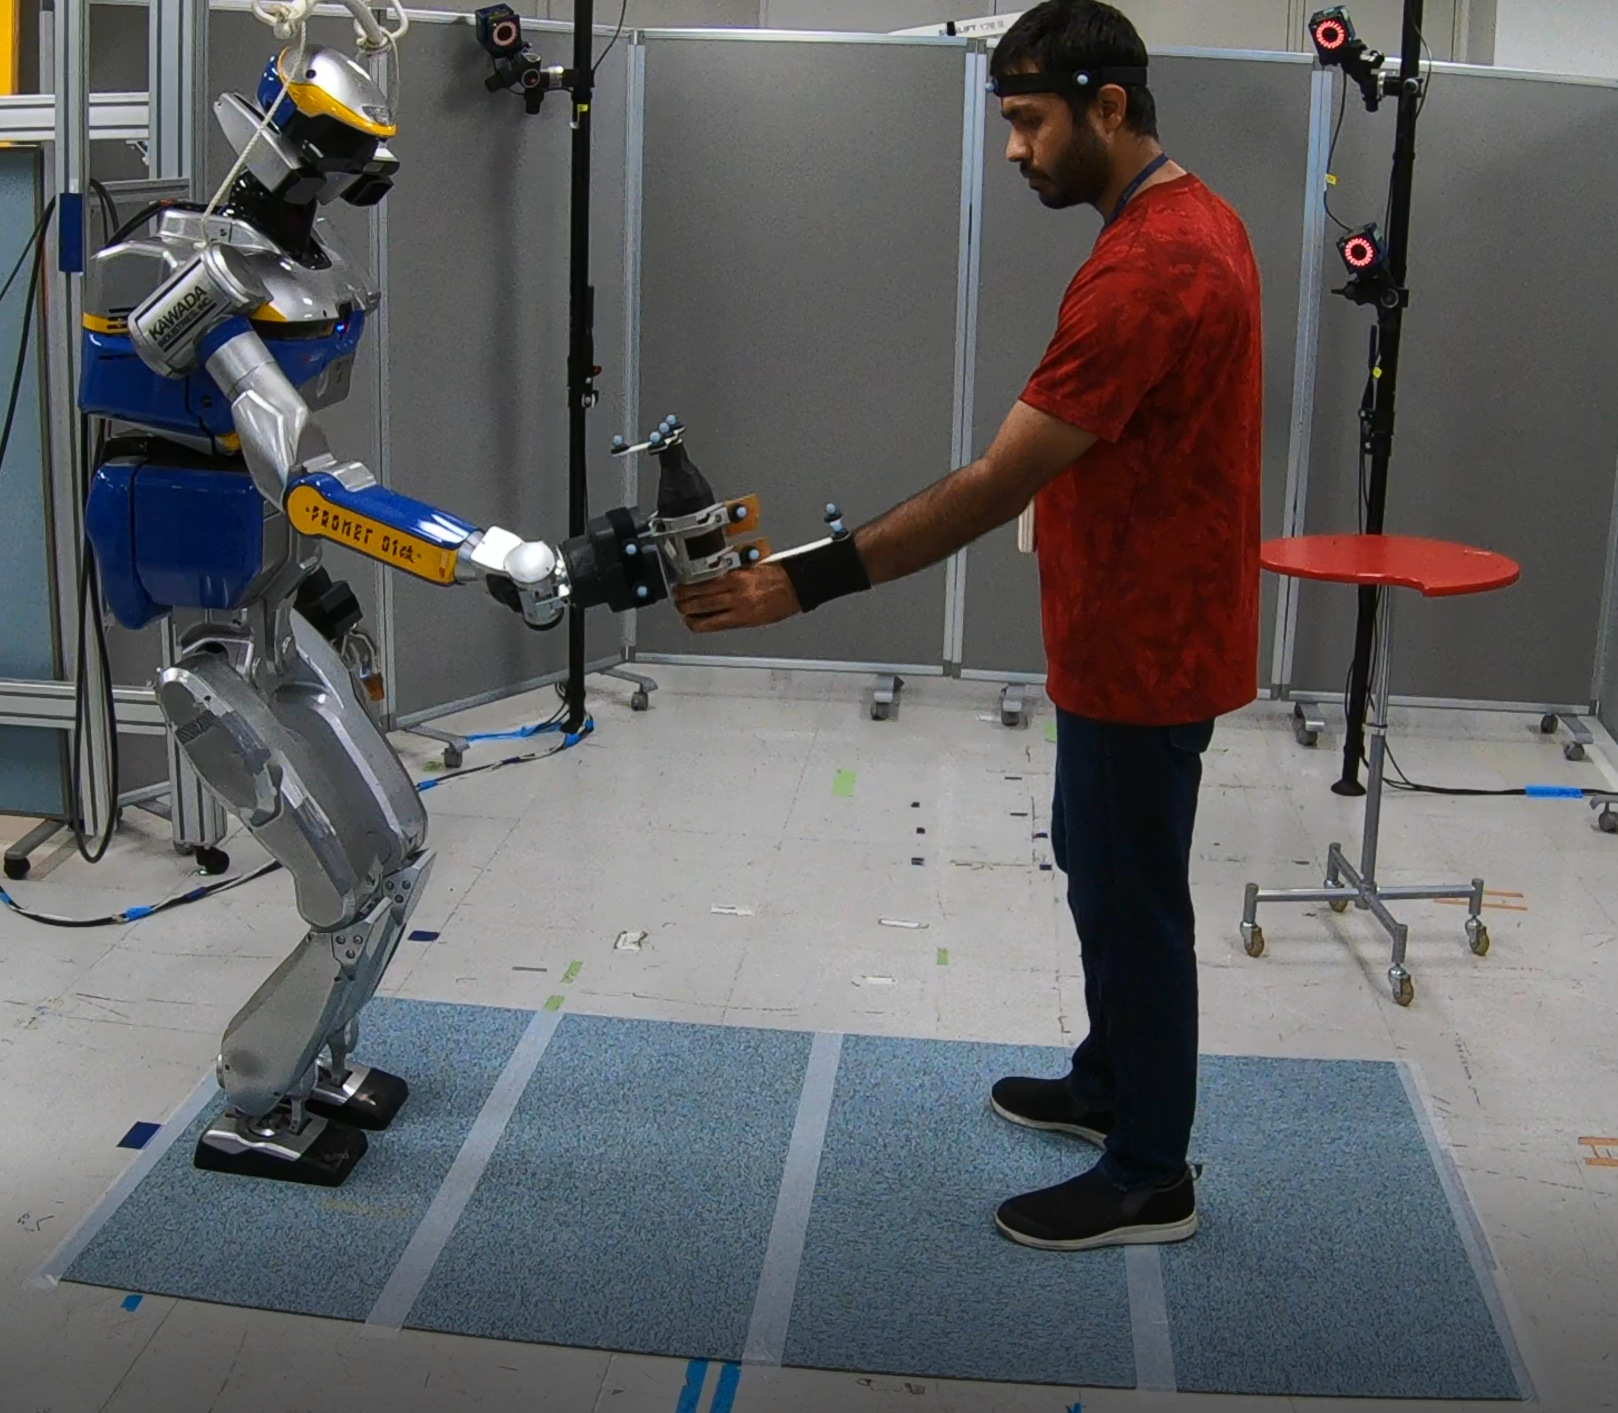
\includegraphics[width=.8\linewidth]{plots/c4-plots/hl-rr}}
	\caption{HRP-2Kai trying to grasp object using right end-effector.}
	\label{fig:markerEf1}
\end{figure} 

We explained further in detail in the subsection (\nameref{FSM}), but before that, we mention another (\nameref{surface wrench}) that we also utilize for closing gripper when the object is in the vicinity.



\subsection{Method 2: surface wrench}\label{surface wrench}

\begin{figure}[ht]
	\centering{\includegraphics[width=0.7\columnwidth]{plots/c4-plots/wrist-surface2}}
	\caption{Virtual intrinsic surfaces (green) on robot wrists.}
	\label{fig:wrist-surface2}
\end{figure}


Just by knowing the relative position of the object \texttt{w.r.t} the robot, end-effector gripper is not enough for safe and reliable object handover. As the lack of anthropomorphic hands and the visual features of the manipulative gripper can be intimidating to some humans. Therefore in conjunction to the mocap marker-based method mentioned earlier we also computed ${}^\text{surf}\vec{f}$, the \textit{gravity-free} force vector in the intrinsic surface frame $surf$ of the gripper (see Fig.~\ref{fig:wrist-surface2}). Let ${}^s\vec{f}\in F^6$ denote the \textit{gravity-free} spatial force vector in the local sensor frame $s$. Note that ${}^s\vec{f}$ has both force and couple components, but we were only interested in the force component. We can easily get the coordinate transformation between the surface frame and force sensor frame, knowing the body at which the force sensor is attached.

\begin{equation}\label{X_s_surf}
    {}^\text{surf}X_{s} = {}^\text{surf}X_{b} {}^{b}X_s
\end{equation}

where, $b$ denotes the body frame at which the force sensor is attached, in our case force sensor(s) are attached to the wrist(s) of HRP-2Kai.

One can generally obtain the transformation matrix for a force vector as explained in~\cite{featherstone2014rigid} if $X$ is responsible for coordinate transformation on motion vectors then using the equation (\ref{X*}), $X^{*}$ would do the same transformation on force vectors since both are related~\cite{featherstone2014rigid},

%%% check page 17-25
\begin{equation}\label{X*}
    X^{*} = X^{-T}
\end{equation}

therefore, force vector in the surface frame $surf$ can be obtained by utilizing equations (\ref{X*}) and (\ref{X_s_surf}), we get

% Dual Coordinates: page 9~\cite{featherstone2014rigid} $X^{*} f$, check page 246 as well
\begin{equation}\label{force surf}
    {}^\text{surf}\vec{f} = {}^\text{surf}X_{s}^{*} {}^s\vec{f}
\end{equation}

where, ${}^\text{surf}X_{s}^{*}$ is the transformation matrix for transformation of force vector from force sensor frame $s$ to gripper intrinsic surface frame $surf$. Finally we measure $\abs{{}^\text{surf}\vec{f}}$ (after removing initial offset) along the gripper's insertion ($z$)-axis, during the interaction between object and gripper just prior to handover during 1$^\text{st}$ \textit{sequence} and if the measured $\abs{{}^\text{surf}\vec{f}}$ is greater than 5N along with the outcome of equation (\ref{area}) then it is safe for robot to close the gripper and hence grasp the object. We further explained complete handover \textit{routine} utilizing above discussed methods in the next subsection (\nameref{FSM}).

\subsection{Finite state machine}\label{FSM}

\begin{figure}[hpt]
	\centering{\includegraphics[width=1\columnwidth]{plots/c4-plots/h-to-r.jpg}}
	\caption{human to humanoid object handover, t1 to t8 transition states.}
	\label{fig:h-to-r}
\end{figure}

The whole handover \textit{routine} is a continuous process but for clarity we have divided it into several transition steps of Finite State Machine (FSM)~\cite{johnson1968automatic}, also (see Fig.~\ref{fig:fsm}) for graphical implementation and Algorithm (\ref{interaction forces}) of (\nameref{handoverAppendix}) as well, the transitions between states are set to be continuous upon the success of previous transition. To understand the interaction forces model, let $\mathcal{\vec{F}}\in \mathbb{R}^3$ denote the current \textit{gravity-free} force sensor reading in the robot frame $\mathcal{R}$. During 1$^\text{st}$ \textit{sequence} of human to robot handover when human holds the object and starts to approach somewhere with the reachable workspace of robot to handover the object (see Fig.~\ref{fig:h-to-r}), in such a situation due to any acceleration of the robot end-effector while approaching towards the object, a wrist force sensor would only show readings due to the inertial forces~\cite{spong2008robot} that are acting on the robot end-effector, which we termed ${}^\text{zero}\vec{\mathcal{F}}$ as force sensor offset reading (see equation~\ref{Fzero}). Let ${}^\text{obj}\overline{\mathcal{F}}\in \mathbb{R}^3$ be the average of contact forces between the end-effector (gripper) and the environment (object) during the resting (${}^{\text{ef}}v=0$) period of robot end-effector along the $xyz$ axes and let ${}^\text{inert}\vec{\mathcal{F}}$ be the inertial force acting on the object due to the acceleration (lets call it ${}^{\text{ef}}a$) of robot end-effector when moving towards the predicted pose of human hand during the 2$^\text{nd}$ \textit{sequence} of handover as shown in (Fig.~\ref{fig:r-to-h}). Let ${}^\text{pull}\vec{\mathcal{F}}$ be the current \textit{minimum} interaction force exerted on the object by the human co-worker and sensed by the robot wrist force sensor while retreating the object during 2$^\text{nd}$ \textit{sequence} of robot to human handover and let ${}^\text{old}T$, ${}^\text{new}T$ $\in \mathbb{R}^3$ be the respective initial default hand-tuned and updated force thresholds. We now explain each state of FSM as shown in (Fig.~\ref{fig:fsm}).


\begin{figure}[hptb]
	\centering
	\begin{tikzpicture}[node distance=5cm, auto, scale = 1, ->,>=stealth, line width=2.3pt, kant/.style={text width=2cm, text centered, sloped}]
	\tikzstyle{cloud} = [draw,ultra thick, circle ,fill=white!20, text width=4em, text centered, node distance=9em, auto, inner sep=0pt, minimum height=1em]
	\tikzstyle{blank} = [circle ,fill=white!20, text width=5em, text centered, node distance=5em, auto, inner sep=0pt, minimum height=2em]
	\tikzstyle{line} = [draw, -latex', inner sep=0pt, minimum height=2em]
	
	\node[cloud,initial above] (human has object) {human has object?};
	\node[cloud, node distance=4cm] (human hand is near?) [right of=human has object] {is object near robot?};
	\node[cloud] (open gripper) [below of=human hand is near?] {open gripper};
	\node[cloud] (stop motion) [right of=open gripper] {maintain current pose};
	\node[cloud] (object inside gripper?) [below of=open gripper] {object inside gripper?};
	\node[cloud] (close gripper) [right of=object inside gripper?] {close gripper};
	\node[cloud] (robot has object) [right of=close gripper] {robot receives object};		
	\node[cloud] (go rest pose) [below of=robot has object] {go to rest pose};
	\node[cloud] (start motion) [left of=go rest pose] {continue motion};
	\node[cloud, node distance=3.8cm] (human hand is near again?) [left of=start motion] {human hand near object?};	
	\node[cloud] (pull handover object) [below of=human hand is near again?] {human pulls object?};
	\node[cloud, node distance=5cm] (open gripper release object) [right of=pull handover object] {gripper releases object};
	\node[cloud] (handover occurred) [below of=open gripper release object] {human receives object};
	\node[cloud, node distance=5cm] (go rest pose2) [left of=handover occurred] {go to rest pose};
	\node[blank] (blank)[left of = go rest pose2]{};
	
	\path[->] (human has object)  edge [loop left]   node  {no} ();
	
	\path [line] (human has object) edge     node[above, kant]{t1, 1$^\text{st}$ \textit{sequence}} (human hand is near?);
	
%	\draw[black,thick,->] (human hand is near?.90) node [above ]{no} arc  (0:240:6mm);
	  \path[->] (human hand is near?)  edge [loop right]   node  {no} ();
 
	
	\path [line] (human hand is near?) edge      node {t2} (open gripper);
	\path [line] (open gripper) edge              node {t3} (stop motion);
	\path [line] (open gripper) edge              node {t4} (object inside gripper?);
	
	\path [line] (object inside gripper?) edge   node {t5} (close gripper);
	 \path[->] (object inside gripper?)  edge [loop left]   node  {no} ();
	
	\path [line, dashed] (close gripper) edge          node [above, kant]{t6, if false close?} (open gripper);
	\path [line] (close gripper) edge         node {t7}(robot has object);
	\path [line] (robot has object)edge        node[left]{t8, ${}^\text{obj}F$} (go rest pose);
	\path [line] (go rest pose) edge           node [above, kant]{t9, 2$^\text{nd}$ \textit{sequence}} (start motion);
	\path [line]  (start motion)edge           node [above, kant]{t10, ${}^\text{inert}F$} (human hand is near again?);
	
	\path [line]  (human hand is near again?)edge  node {t11, ${}^\text{pull}F, {}^\text{new}T$}  (pull handover object);
	 \path[->] (human hand is near again?)  edge [loop left]   node  {no} ();
	
	\path [line]  (pull handover object)edge       node [below, kant]{t12, ${}^\text{pull}F >{}^\text{new}T$} (open gripper release object);
	\path[->] (pull handover object)  edge [loop left]   node  {no} ();
	
	\path [line]  (open gripper release object)edge  node {t13}(handover occurred);
	\path [line]  (handover occurred)edge           node {t14}(go rest pose2);
	\path [line, dashed]  (go rest pose2) -|       node [near end, above, rotate=90]{t0, \textbf{restart handover}}(human has object);
	
	\end{tikzpicture}
	\caption{Overview of human humanoid object handover Finite-State-Machine (FSM)}
	\label{fig:fsm}
\end{figure}


\begin{figure}[hpt]
	\centering{\includegraphics[width=1\columnwidth]{plots/c4-plots/r-to-h.jpg}}
	\caption{humanoid to human object handover t9 to t14 transition states.}
	\label{fig:r-to-h}
\end{figure}

\begin{enumerate}[start=0,label={\bf{t}\arabic*:}]

    \item $\norm{{}^h{P} - {}^\text{obj}{P}} < 0.02$\\
    We start FSM under the assumption that the human co-worker is already grasping the object, and he/she is ready with the intention of handover. ${}^h{P}$ is the position of point $A$ on the ${\bf L}$ shape body as the human hand marker position (see Fig.~\ref{fig:lshapes}).
    
    
    \item $\norm{{}^h{P} - {}^{\text{ef}}{P}} < 0.10$\\
    During 1$^\text{st}$ \textit{sequence} of handover \textit{routine}, i.e. human to robot object handover. We measure the relative position of human hand and robot end-effector mocap markers, the state transition is successful if the euclidean distance $d$ is less than 0.1 meters, where $d = \norm{{}^h{P} - {}^{\text{ef}}{P}}$. ${}^{\text{ef}}{P}$ is the average position of gripper tips marker ${}^\text{ga}P, {}^\text{gb}P$. 
    
    \item Open Gripper\\
    The robot opens the gripper and presents with its intention to grasp the object.
    
    \item $\norm{{}^h{P} - {}^{\text{ef}}{P}} \leq 0.05$, maintain current pose\\
    To avoid collision between robot end-effector and human hand we reduce the end-effector velocity (${}^{\text{ef}}v\simeq0$) when the interaction distance $d = \norm{{}^h{P} - {}^{\text{ef}}{P}}$ is less than 0.05 meters. We also measure ${}^\text{zero}\vec{\mathcal{F}}$ as force sensor offset during this time.
    
    \begin{equation}\label{Fzero}
    {}^\text{zero}\vec{\mathcal{F}} = {\vec{\mathcal{F}}}
    \end{equation}
    
    \item (${}^\text{surf}\vec{f}(z) \geq 5N) \quad $ \& $ \quad (f({}^\text{obj}\vec{P})  == 1$)\\
    We declare robot is ready to close the gripper when the object is inside gripper if output of equations (\ref{area bool},~\ref{force surf}) satisfy together.
    
    \item Close Gripper\\
    Let ${}^\text{close}\vec{\mathcal{F}}$ be the measured force reading at the timing of closing gripper.
        
    \begin{equation}\label{Fclose}
	    {}^\text{close}\vec{\mathcal{F}} = \vec{\mathcal{F}}
    \end{equation}
    
    Robot closes gripper; presumably, the object is grasped as well. However, it is easy to check whether the robot grasps the object or if it is a false close. It is safe to say that its a false close if output of equation (\ref{area bool}) is $0$, along with the condition $\norm{{}^\text{zero}\vec{\mathcal{F}}-{}^\text{close}\vec{\mathcal{F}}} \simeq{0}$, since these are same measured force sensor offsets. Therefore, in such scenario next transition state would be \textbf{t6} to open gripper and repeat, otherwise \textbf{t7}, as shown in (Fig.~\ref{fig:fsm}).
   
   \item Open Gripper due to false close, otherwise,
   
   \item This transition confirms that the robot receives the object and now the object \textit{mass} can be calculated based on the forces measured during previous states.
   
   \begin{equation}
   {}^\text{obj}\overline{\mathcal{F}} = \frac{1}{n}\sum_{i=1}^{i=n} \vert{ (\vert{\vec{\mathcal{F}}}\vert - \vert{{}^\text{zero}\vec{\mathcal{F}}}\vert) }\vert
   \end{equation}
   
   ${}^\text{obj}\overline{\mathcal{F}}$, is pure force sensor reading when ${}^{\text{ef}}a=0$ and object is grasped by the robot, $n$ is the low-level controller time-step counter that increments every $5$ ms (see subsection~\nameref{QPController}), before transitioning to next state, we intentionally stay on this state for 1 second i.e. until $i==200$ to measure the average of ${}^\text{obj}\vec{\mathcal{F}}$ over 200 samples. Finally, object $mass$ can be obtained using equation (\ref{obj mass}).
   
   \begin{equation}\label{obj mass}
   objMass = \norm{{}^\text{obj}\overline{\mathcal{F}}}/9.80665
   \end{equation}
   
   \item Go to rest pose \\
   Both human and robot return to their resting posture, with the robot carrying the object. This ends the 1$^\text{st}$ \textit{sequence} of handover.
   
   \item 2$^\text{nd}$ \textit{sequence} begins\\
   Robot to human object handover. The robot continues to predict human hand position and moves towards it when the human co-worker approaches somewhere within the robot's reachable workspace. During this time, we measure the ${}^\text{inert}\vec{\mathcal{F}}$ inertial force acting on the object due to the acceleration of end-effector.
   
   \begin{equation}
   {}^\text{inert}\vec{\mathcal{F}}  = objMass * {}^{\text{ef}}\overline{a}
   \end{equation}
   
   Where, ${}^{\text{ef}}\overline{a}$, is the average acceleration of the robot end-effector.
   
   \item $\norm{{}^h{P} - {}^{\text{ef}}{P}} < 0.05$\\
   Once again, we measure the relative position of human hand and robot end-effector mocap markers, the state transition is successful if the euclidean distance $d = \norm{{}^h{P} - {}^{\text{ef}}{P}}$ is less than 0.05 meters. That means human is ready with the intention to grasp the object.
   
   \item Human attempts to retrieve the object
   
   \begin{equation}
   {}^\text{pull}\vec{\mathcal{F}} = \vert{ (\vert{\vec{\mathcal{F}}\vert} - \vert{{}^\text{inert}\vec{\mathcal{F}}}\vert - \vert{{}^\text{zero}\vec{\mathcal{F}}}\vert) }\vert
   \end{equation}
   
   \begin{equation}
   {}^\text{new}\vec{T} = {}^\text{obj}\overline{\mathcal{F}} + {}^\text{old}\vec{T}
   \end{equation}
   
   where, ${}^\text{old}\vec{T}$ was hand tuned after several attempts with multiple objects. Default ${}^\text{old}\vec{T}$ values were set to $[6, 6, 6]$ N, after some preliminary trials. 
   
   \item Open Gripper, human grasps the object if both below conditions satisfy
   
   \begin{equation}\label{Fpull}
   \begin{cases}
   \norm{{}^h{P} - {}^\text{obj}{P}} < 0.02  \\
   {}^\text{pull}\vec{\mathcal{F}}\geq {}^\text{new}\vec{T}, & \lor x, \lor y, \lor z
   \end{cases}
   \end{equation}
   
   where, $\norm{{}^h{P} - {}^\text{obj}{P}}$ is again euclidean distance between human hand and object mocap markers.
   
   \item Object returns to the human co-worker, human retreats.
   
   \item End of 2$^\text{nd}$ \textit{sequence} of handover.\\
   Both human and robot returns to their resting posture, with human carrying the object (see Fig.~\ref{fig:halfsit}).
    
\end{enumerate}

Finally, this ends the object handover \textit{routine} between human and robot co-workers. Afterwards, we again repeat the handover \textit{routine}, starting with 1$^\text{st}$ \textit{sequence} of handover.



\section{Either hand generalized handover}\label{both hands individual}

As mentioned in an earlier section (\nameref{handover routine}), up till now we have discussed human-robot bi-directional object handover under the scenario where robot always uses its left end-effector, and human always uses his/her right hand. However unlike several handover studies in the past~\cite{cakmak2011human, medina2016human, huber2008Indus, kupcsik2016learning}, we can take the benefit of having a humanoid at our disposal; therefore we further generalize our human-humanoid bi-directional object handover \textit{routine} and extend it by exploiting either human left or right hand and similarly left or right end-effector of robot. Basically we extended our one-handed handover \textit{routine} into four possible scenarios (see Fig.~\ref{fig:handover scenarios}) such as,

\begin{enumerate}
	\item robot left end-effector $R_\text{efl}$ $\longleftrightarrow$ human right hand $H_r$
	\item robot left end-effector $R_\text{efl}$ $\longleftrightarrow$ human left hand $H_l$
	\item robot right end-effector $R_\text{efr}$ $\longleftrightarrow$ human left hand $H_l$
	\item robot right end-effector $R_\text{efr}$ $\longleftrightarrow$ human right hand $H_r$
\end{enumerate}


\begin{figure}[hpt]
	\centering
	\begin{tikzpicture}[node distance=5cm, auto, scale = 1, ->,>=stealth, line width=2.3pt, kant/.style={text width=2cm, text centered, sloped}]
		\tikzstyle{cloud} = [draw,ultra thick, circle ,fill=white!20, text width=4em, text centered, node distance=9em, auto, inner sep=0pt, minimum height=1em]
		\tikzstyle{line} = [draw, -latex', inner sep=0pt, minimum height=2em]
		
		\node[cloud] (obj) {object};
		\node[cloud] (hl) [below left of = obj] {$H_l$};
		\node[cloud] (hr) [below right of= obj] {$H_r$};

		\node[cloud] (rr) [below of = hl] {$R_\text{efr}$};
		\node[cloud] (rl) [below of= hr] {$R_\text{efl}$};

		\path [line] (obj) edge  node[above, kant]{} (hl);
		\path [line] (obj) edge  node[above, kant]{} (hr);		
		
		\path [line] (hl) edge  node[above, kant]{} (rl);
		\path [line] (rl) edge  node[above, kant]{} (hl);
	
		\path [line] (hl) edge  node[above, kant]{} (rr);
		\path [line] (rr) edge  node[above, kant]{} (hl);
	
		\path [line] (hr) edge  node[above, kant]{} (rl);
		\path [line] (rl) edge  node[above, kant]{} (hr);
		
		\path [line] (hr) edge  node[above, kant]{} (rr);
		\path [line] (rr) edge  node[above, kant]{} (hr);

	\end{tikzpicture}
	\caption{Possible handover scenarios between human and humanoid.}
	\label{fig:handover scenarios}
\end{figure}


In this section we will only mention changes that need to be incorporated into the previous sections for the generalization and extension of previously stated handover \textit{routine} to cover above four possible scenarios (Fig.~\ref{fig:handover scenarios}). We mainly modify here parameters of FSM states during transitions {\bf t0, t1} and {\bf t10}, which are already discussed in detail (see subsection~\nameref{FSM}). Again we assumed a human is ready to handover the object if he/she is holding it in his/her either hand. We have also assumed that just like many humans, our robot also acts like a \textit{right-handed} `person', therefore robot right end-effector would get priority over left in case object is at relatively same distance from both end-effectors or in case where the handover predicted position is at or converging towards the centre of robot body. This hand preference is mainly due to a recent study~\cite{han2013quantifying}, which showed that right-handed people tend to prefer the right over left hand when they have the choice of pointing at a target location that is almost equally distant between both hands.


In this framework, the choice or preference of employing end-effector (either left or right) by the robot co-worker is based on the shortest relative distance of object to either human hand, which can be determined by using equation (\ref{human obj dist}) along with together the direction (mainly along $y$-axis) and shortest relative distance of \textit{that} active human hand with respect to both end-effectors, as per equations (\ref{human hand dir} and~\ref{robot obj dis}) respectively. For example, if human is holding object in his/her right hand ${}^\text{hr}{P}$ and if the estimated predicted position of his/her hand (see section~\nameref{prediction_model}) is converging somewhere in the negative $y$-coordinate space, then robot right end-effector ${}^\text{efr}{P}$ would be utilized to receive the object during handover as shown in (Fig.~\ref{fig:hr-to-rr}).


\begin{figure}[hpt]
	\centering{\includegraphics[width=0.7\columnwidth]{plots/c4-plots/hr-rr}}
	\caption{Object handover between human right hand and HRP-2Kai right end-effector.}
	\label{fig:hr-to-rr}
\end{figure}


\begin{equation}\label{human obj dist}
\centering
\begin{cases}
	\norm{{}^\text{hl}{P} - {}^\text{obj}{P}} < \norm{{}^\text{hr}{P} - {}^\text{obj}{P}}, & \text{human left hand (${}^\text{hl}{P}$)}  \\
	\\
	\norm{{}^\text{hl}{P} - {}^\text{obj}{P}} > \norm{{}^\text{hr}{P} - {}^\text{obj}{P}}, & \text{human right hand (${}^\text{hr}{P}$)}
\end{cases}         
\end{equation}


\begin{equation}\label{human hand dir}
\centering
\begin{cases}
\norm{{}^{h}{P}(y)} > 0.1,  &  \text{robot left end-effector (${}^\text{efl}{P}$)} \\
\\
\norm{{}^{h}{P}(y)} \leq 0.1,  &  \text{robot right end-effector (${}^\text{efr}{P}$)}
\end{cases}         
\end{equation}

\begin{equation}\label{robot obj dis}
\centering
\begin{cases}
\norm{{}^{h}{P} - {}^\text{efl}{P}} < \norm{{}^{h}{P} - {}^\text{efr}{P}}, &  \text{robot left end-effector (${}^\text{efl}{P}$)} \\
\\
\norm{{}^{h}{P} - {}^\text{efl}{P}} > \norm{{}^{h}{P} - {}^\text{efr}{P}}, &  \text{robot right end-effector (${}^\text{efr}{P}$)}
\end{cases}
\end{equation}


Where ${}^{h}{P}$ in equations (\ref{human hand dir} and~\ref{robot obj dis}) could be either of the human hand position depending upon equation (\ref{human obj dist}). However in cases where there is a switching of object in between human hands and within the 1$^\text{st}$ \textit{sequence} of handover, such as in some rare case human co-worker may decide to move the object from his/her left to right hand or vice-versa for any reasons, under those conditions we rely on the effect of \textit{hysteresis} for robot to decide whether it needs to switch end-effector or continue uninterruptedly. But note that we do not consider the problem of object handover in-between robot end-effectors, therefore once the object is being handed over to the robot co-worker, i.e. during 2$^\text{nd}$ \textit{sequence}, then the robot would not be able to switch its end-effector, however the human co-worker is still free to choose either of his/her hand to grasp the object back. Using the earlier example where human co-worker right hand has the object, and his/her position is converging somewhere in the negative $y$-coordinate space. While during the 1$^\text{st}$ \textit{sequence} of handover if human switches the object in-between his/her hand ---say from right to left hand, then by taking recent history (direction) of human hand into account we further utilize the outputs of equations (\ref{human hand dir} and~\ref{robot obj dis}) to measure change in the direction of human hand and its shortest relative distance from the end-effectors, and based on these observations robot decides to act accordingly. By exploiting \textit{hysteresis} effect, we make sure that robot does not respond abruptly to changes made by the human.


%\clearpage

\section{Bi-manual handover}\label{both hands together}

It is very natural between humans to use both hands to manipulate a heavy or large shape object to gain confidence and maintain stability during a physical interaction or even while performing a collaborative task. Using both hands together during handing over such an object to one another is no different. Similarly, in scenarios where the use of the single hand is not enough or feasible to perform safe and reliable handover of a large, heavy object between human and humanoid co-workers, then it should also be an obvious choice for the robot as well to use both hands together whenever necessary. 


Here, we extend the handover \textit{routine} under the scenario of bi-manual large object transfer between human and humanoid co-workers. We formulate this handover \textit{routine} in a manner such that human co-worker is allowed to use either or both hands to handover/receive the object to/from robot co-worker. However, the robot would always use both hands while receiving and returning of such object, given the physical, structural properties of the object.


\subsection{Handover object(s)}


\begin{figure}[hpt]
	\centering{\includegraphics[width=0.8\columnwidth]{plots/c4-plots/handoverPipe}}
	\caption{Hollow cylinder shaft as object for bi-manual handover between human humanoid. Subplot A) shows inner and outer radius of the hollow cylinder and placement of the $\bf L $ body shape with $o$. Subplot B) shows representation of our method to get the offset for safe handover location.}
	\label{fig:pipe_ex}
\end{figure}


The object(s) (two of them) we chose to handover between human-humanoid dyads are cylindrical (see Fig.~\ref{fig:pipe_ex}). We chose these objects purely for simplicity and demonstration purposes in this study. Though our handover model would practically work on several distinguishable objects as long as the object's basic physical, structural properties are known; however, the mass of the object is optional. The cylindrical structures we used are hollow yet quite rigid. The inner $r_i$ and outer $r_o$ radii for those two objects are \textins{$0.055$, $0.065$} m and \textins{$0.07$, $ 0.08$} m respectively, lengths $l$ are \textins{$0.90$, $ 0.12$} m, and the mass of objects are \textins{$0.40$, $1.1$} kg, again we don't need to know mass of object in advance as it can be computed during handover \textit{routine} when robot carries the object as already explained earlier in the subsection (\nameref{FSM}).


\begin{figure}[hpt]
	\centering{\includegraphics[width=0.7\columnwidth]{plots/c4-plots/robot_has_pipe}}
	\caption{HRP-2Kai using both end-effectors to manipulate handover object based on the human hand relative orientation.}
	\label{fig:pipe_ori}
\end{figure}


Here as well we have placed a ${\bf L}$ shape rigid body at the centre of the object as shown in (Fig.~\ref{fig:pipe_ex} and Fig.~\ref{fig:pipe_ori}) with respective $xyz$ local coordinate axes in local frame $o$ and are along the direction of robot frame axes. The object pose (position and orientation) is given by ${}^{o}{X}_M$ (see equation~\ref{X_M_o}). Also object orientation can be formulated similarly to human hand orientation, as explained earlier in section (\nameref{orientation_model}).


\subsection{Constraint motion}

Following is an overview of constraint motion during handover \textit{routine} using both hands and end-effectors.
\begin{compactitem}
	\item Human moves with the intention to handover the object.
	\item Both robot end-effectors approaches towards the object.
	\item Robot receives the object.
	\item Contacts are established between robot grippers and object surfaces.
	\item The contact constraint governs robot end-effectors motion under null velocity.
	\item Robot end-effectors follows the dominant human hand under the contact constraint.
\end{compactitem}

Here we approach differently during the 1${}^\text{st}$ and 2${}^\text{nd}$ \textit{sequence}s of handover. During the 1${}^\text{st}$ \textit{sequence} of object handover from human to humanoid, we predict and estimate both human hands positions individually along with estimating the object orientation. Specifically, we use unique \texttt{position} and \texttt{orientation} tasks (see subsection~\nameref{QPTasks}) to move each of the robot end-effector to the desired handover location. Once the object is handed over to the robot co-worker and after grasping it using both end-effectors, we remove the \texttt{position} and \texttt{orientation} tasks on one of the end-effector at the beginning of 2${}^\text{nd}$ \textit{sequence} because of the kinematic contact constraints (see subsection~\nameref{QPConstraints}) imposed by the object. 

Now we would first introduce contact surfaces and kinematic constraints before explaining the simultaneous motion of the robot end-effectors due to constraints imposed by the object during 2$^\text{nd}$ \textit{sequence} of handover \textit{routine}.

\begin{figure}[hptb]
	\centering{\includegraphics[width=1\columnwidth]{plots/c4-plots/grippers-intern}}
	\caption{Robot grippers with graspable internal surfaces.}
	\label{fig:gripper-intern}
\end{figure}


\paragraph*{Contact surface(s)} 

The contact surfaces or surface patches were initially defined on the palm of each gripper in advance. Grippers local frame are shown in (Fig.~\ref{fig:gripper-intern}). The contacts are established, when during the handover \textit{routine} the robot grasps the object and its grippers internal surface come in contact with the object's graspable surface. These contacts are necessary to move freely or limit the motion of end-effectors in one or more direction (3 \texttt{x} translation or 3 \texttt{x} rotation)~\cite{bouyarmane2018multi}. Thus robot may lose one or more degrees of freedom (DOF) in motion due to the constraints introduced by the object's body.


\paragraph*{Contact kinematics and constraint}

To allow the concurrent motion of the robot end-effectors and the object, contacts are defined as the kinematic constraints in the (\nameref{QPController}), specifically we used the \textit{fixed} contact mode, as defined by the~\cite{balkcom2002computing}, where all six degrees of freedom are constrained (no translation, no rotation at contact) which restricts and prevents any possibility of sliding motion between the robot end-effectors and the object. Lets consider $b_{l}$, $b_{r}$ and $b_o$ be the respective left, right end-effectors and object bodies and let $v_i$ be the $i$-th body velocity. Let $j_l$, and $j_r$ be the two joints under the kinematic constraint between these bodies. Such that, the relative joint velocities $v_\text{jl}$ and $v_\text{jr}$ between these bodies in contact would be given by the set of equations (\ref{joint_vel})~\cite{Featherstone:1987} and therefore the velocity constraints between these bodies would be given by the set of equations (\ref{vel_const}) \cite{ohwovoriole1980externsion} (see also subsection~\nameref{QPConstraints}). We later introduce this velocity constraint to the (\nameref{QPController}).

\begin{equation}\label{joint_vel}
\centering
\begin{cases}
v_\text{jl} = v_\text{bl} - v_\text{bo} \\
v_\text{jr} = v_\text{br} - v_\text{bo} \\
\end{cases}
\end{equation}

\begin{equation}\label{vel_const}
\centering
\begin{cases}
J_\text{lo}(v_\text{bl} - v_\text{bo}) = 0\\
J_\text{ro}(v_\text{br} - v_\text{bo}) = 0\\
\end{cases}
\end{equation}

where, $J_\text{ik}$ is the Jacobian matrix of all points of contact forces between $i$-th body and $k$-th body.


\paragraph*{1$^\text{st}$ \textit{sequence}: before object-robot contacts}

Under the handover \textit{routine} scenarios, we initiate handover 1$^\text{st}$ \textit{sequence} when human holds the object and start approaching somewhere within the reachable workspace of the robot — assuming that he/she is ready with the intention to handover the object to the robot. The human can grasp the object with any possible comfortable orientation using either left/right or both hands simultaneously and any place on the object's surface along its length. The only constraint we put while holding/grasping object was not to occlude the ${\bf L}$ shape body and mocap markers on it (see Fig.~\ref{fig:h-r-pipe-handover} for such possible pose(s)).


\begin{figure}[hptb]
%	\centering{\includegraphics[width=0.7\columnwidth]{plots/c4-plots/h-r-pipe-handover}}
	\centering{\includegraphics[width=0.7\columnwidth]{plots/c4-plots/h-r-pipe-handover1}}
	\caption{Bi-manual object handover between human and humanoid using both human hands and both end-effectors.}
	\label{fig:h-r-pipe-handover}
\end{figure}

Compared to the one-handed handover scenario, which was discussed in previous section (\nameref{both hands individual}), here during human to robot co-worker object handover \textit{sequence} instead of just predicting human hand positions individually like earlier, we also measure the Euclidean distances of each human hand on the object's surface \texttt{w.r.t} the object's centre using the following set of equations (\ref{hand rel pos on obj}). These distances act as an offset correction to the predicted positions of human hands, along the length of the object. These offsets are essential as they allow the robot to find safe and optimum positions on the object's surface to grasp. Also, while making sure end-effectors stay quite away from the human hands occupied the object's surface (see Fig.~\ref{fig:h-r-pipe-handover}). Moreover, it avoids any possible head-on collision between the end-effectors and the human hands when the robot tries to approach and grasp the object.


Initially, we predict and estimate human hand positions by utilizing previously discussed prediction model from section (\nameref{prediction_model}). Given the object shape and its structural properties (in our case length of cylindrical shaft), the offsets along object's length can be calculated using set of equations (\ref{hand rel pos on obj}) in the object local frame $o$ (see Fig.~\ref{fig:pipe_ex} B) from the center in both directions. This offset is then further transformed into the robot frame and finally added to the already predicted position of the human hands \texttt{w.r.t} robot end-effectors using equation (\ref{offset_transform}).



\begin{equation}\label{hand rel pos on obj}
\centering
\begin{cases}
a = \norm{{}^\text{obj}{P} - {}^{h}{P}} & \text{}  \\

b = \abs{l/2 - a}  & \text{} \\
\\
{}^\text{off}{d} = \pm 2*a/3 &  \text{if} \; a \geq b \; $ \& $ \; a\leq l/2\\

{}^\text{off}{d} = \mp 2*b/3 &  \text{if} \; a < b \; $ \& $ \; a\leq l/2\\
\end{cases}
\end{equation}

where, ${}^\text{obj}{P}$ is the centre position given by the mocap marker at its centre, $a$, $b$ and ${}^\text{off}{d}$ are the euclidean distances, which provides grasped location of human hands on the object surface from its centre. Using this crucial information robot can estimate possible points on the object's surface, which are available to be grasped during the handover. Here, $h$ in ${}^{h}{P}$ represents either left $H_l$ or right $H_r$ human hand and the sign of ${}^\text{off}{d}$ depends on the choice of left or right human hand (see Fig.~\ref{fig:pipe_ex} B). Let $\hat{u} = \{0, 1, 0\}$ be the free unit vector along the length of the object, i.e. along the $o_y$-axis of local frame $o$, therefore offset position vector in object frame would be given by


\begin{equation}
	{}^\text{off}{P}_{o} = {}^\text{off}{d} \: \hat{u}  =  \{0, {}^\text{off}{d}, 0\}
\end{equation}


We know for sure that without these offsets, robot end-effectors would inevitably collide with the human hands. Since our prediction model is estimating and predicting the positions of both human hands. Therefore, we need to introduce these offsets in the predicted positions of human hands relative to robot end-effectors. We start by measuring these offsets continuously and from the beginning of handover $\textit{sequence}$. This allowed the robot to adjust while approaching the object, depending on the human hands grasped location on the object's surface. We can obtain the modified predicted positions based on these offsets using Pl\"ucker transformation. We transformed offset position ${}^\text{off}{P}_{o}$ from object frame to mocap frame ${}^\text{off}{P}_{M}$ by below equation (\ref{offset_transform}). Please note, above offset correction method is also valid during the 2$^\text{nd}$ \textit{sequence} of handover when robot holds the object and approaches towards the human decided handover location.


Note here, we considered predicted position of the human hand, but to relatively orient robot end-effectors, we considered the orientation of object but not the human hand(s). In this example of a cylindrical object, the orientation of human hand and object is similar however to generalize this for other possible distinguishable shape objects; it is crucial to consider object's orientation instead of the human hand. As for the other shape objects relative human hand's orientation to grasp the object may not be feasible to perform by the robot. 

%\begin{equation}\label{offset_transform}
%{}^\text{off}{X}_{M} = {}^\text{off}{P}_{o} {}^{o}\mathcal{O}_M
%\end{equation}

\begin{equation}\label{offset_transform}
{}^\text{off}{X}_{M} = 
{}^\text{off}{P}_{o}
 \left[\begin{array}{cc}
{}^{o}\mathcal{O}_M & {}^{h}\mathcal{P}_M(i_\text{predict})
\end{array}\right]
\end{equation}


where, ${}^{o}\mathcal{O}_M$ provides the orientation of object in the mocap frame (see equation~\ref{X_M_o}) and ${}^{h}\mathcal{P}_M$ is the predicted position of human hand(s). Finally, using equation (\ref{offset_transform}), we can replace translation and orientation components of ${}^{h}{X}_M$ in the equation (\ref{X_ef_ht}) with ${}^\text{off}{X}_{M}$, therefore new pose of the handover location relative to the robot end-effectors would be given by

\begin{equation}
	{}^{\text{off}}{X}_{\text{ef}} =  {\bf{}^{\text{\bf off}}{X}_M}  {}^{M}{X}_R {{}^{\text{ef}}{X}_R}^{-1}
\end{equation}
%	{}^{h}{X}_{\text{ef}}(\text{off}) =  {\bf{}^{\text{\bf off}}{X}_M}  {}^{M}{X}_R {{}^{\text{ef}}{X}_R}^{-1}


Finally, at the handover location, we measure the $\abs{{}^\text{surf}\vec{f}}$ (after removing initial offset) forces along the both gripper's insertion ($z$)-axes during the interaction between object and gripper just before handover. Handover occurs when $\abs{{}^\text{surf}\vec{f}}$ exceeds 5N on both end-effectors along with the set of following conditions in equation (\ref{min_posErr_vel}) satisfy for both robot end-effectors.



\paragraph*{2$^\text{nd}$ \textit{sequence}: after object-robot contacts}

So far we have discussed estimating and predicting object handover pose for the robot end-effectors during the 1${}^\text{st}$ \textit{sequence} of handover \textit{routine}. Up till now, each robot end-effector motion was controlled by its own \texttt{position} and \texttt{orientation} task. During the 2$^\text{nd}$ \textit{sequence} of handover \textit{routine} after the contacts have been established between the robot grippers and the object surfaces. Also, because of the introduction of kinematic constraints imposed by the object on the end-effectors, the robot cannot move its end-effectors individually. The successive motion of the end-effectors is therefore now governed by the \texttt{contact constraint} that we introduce to the robot's low-level QP controller. This constraint maintains the contacts between the object and the robot grippers surfaces all the time and the concurrent motion of the end-effectors is made possible by targeting a null velocity constraint with the target objective $\mathscr{I}_\text{contact}=0$ at the contact joints between the object and the end-effectors, see equation (\ref{vel_const}). The \texttt{contact constraint} is already explained at the beginning of this section and also in the subsection (\nameref{QPConstraints}).

As already mentioned earlier, the human co-worker is allowed to use either (both) hand(s) to handover/receive the object to/from robot co-worker. Therefore, when the human starts approaching somewhere within the reachable workspace of the robot to receive the object. We utilized equation (\ref{robot_rel dis}) to select the dominant human hand, mainly by measuring the relative distances between the robot end-effectors and the human hands. We check this condition only once at the beginning of the 2$^\text{nd}$ \textit{sequence} of handover \textit{routine} after the human hand(s) arrive within the reachable workspace of the robot.

\begin{equation}\label{robot_rel dis}
\centering
\begin{cases}
\norm{{}^\text{hr}{P} - {}^\text{efl}{P}} < \norm{{}^\text{hl}{P} - {}^\text{efr}{P}}, &  \text{robot left end-effector (${}^\text{efl}{P}$)} \\
\\
\norm{{}^\text{hr}{P} - {}^\text{efl}{P}} > \norm{{}^\text{hl}{P} - {}^\text{efr}{P}}, &  \text{robot right end-effector (${}^\text{efr}{P}$)} \\
\end{cases}
\end{equation}

Where, ${}^\text{hl}{P}$ and ${}^\text{hr}{P}$ are the position vectors of the respective left and right human hand. Depending on the choice of the dominant human hand, for example, if the left human hand is selected then we remove the \texttt{position}, and \texttt{orientation} tasks of the left end-effector and therefore the motion of this end-effector is now governed using the \texttt{contact constraint} by targeting the null velocity. By doing this, the robot right end-effector would lead the motion by predicting and estimating the pose of the dominant human hand. The problem of predicting and estimating human hand pose can now be treated similarly to the one-handed handover \textit{routine} as mentioned in the section (\nameref{both hands individual}). Please note, set of equations (\ref{hand rel pos on obj}) is also valid to calculate the offset position of end-effector when robot predicts and approaches towards the handover location chosen by the dominant human hand. We just need to replace the human hand position vector ${}^{h}{P}$ with the end-effector position vector ${}^{\text{ef}}{P}$. Where $\text{ef}$ in ${}^{\text{ef}}{P}$ is either left $\text{efl}$ or right $\text{efr}$ end-effector.


Finally, a handover occurs when the set of conditions in the equation (\ref{Fpull}) satisfy for both end-effectors (see~\nameref{FSM}). Note that the conditions in the equation (\ref{Fpull}) are valid only if a human tries to pull the object from the robot. After the robot grippers release the object, we also remove the null velocity \texttt{contact constraint} between the end-effectors and the object surfaces, and add again the previously removed \texttt{position} and \texttt{orientation} tasks to that end-effector. This completes bi-manual handover \textit{routine}.

%\clearpage

\section{Locomotion and handover}\label{locomotion}

A broad general definition of locomotion describes it as an ability to move from one place to another, that could be achieved either by walking, running, jumping and more. Though we are mainly interested in the walking locomotion of a \textit{floating} base robots such as our HRP-2Kai in the context of the object handover between human and robot co-workers. However, after a thorough search of state-of-the-art research in the related field, none of the previous work on the human-robot dyad considered object handover and `walking' in a single framework using a \textit{biped} humanoid platform such as HRP-2Kai. Therefore in order for the robot to be sufficiently proactive, we believe it is essential to consider the possibility of a robot taking a step or two to handover or exchange an object with the human co-worker, in scenarios where short-distance travel is required, to eventually extend robot's reachable workspace. Note that we consider the problem of taking a few steps to handover/receive the object rather than motion planning and navigation.

Some previous studies on human-human dyad object handover have demonstrated that we humans are surprisingly able to predict where our partner would handover an object, often without an explicit communication~\cite{kato2018humans, kato2019handovers}. However we came across one of such study~\cite{hansen2017human}, results of which had shown that we humans often handover an object at the middle of our interpersonal distances~\cite{hall1966proxemic, strabala2013toward}.

Up till now, we formulated our handover problem under the scenario that both human and especially robot co-worker base (feet) are stationary on their respective position in the world frame, such that object handover can happen just by extending their arms. Next in this section, we further extended our handover problem and added another dimension in which robot takes a step(s) (we call it \textit{step-walk}) to handover or receive the object from the human co-worker based on the interpersonal distance between them. We have tested this scenario during both when human-robot dyad uses either one hand or both hands simultaneously.


\subsection{Walking pattern generator}

Though there are many state-of-the-art methods available to generate walking pattern for humanoids, however in this study for step-walk locomotion, we primarily chose to adopt walking pattern generator (WPG) based on the Linear Inverted Pendulum Mode (LIPM) which was designed and tested in our group~\cite{ kajita20013d, caron2016humanoids} along with its native stabilizer~\cite{kajita2010biped, caron2018stair}. 

The goal of WPG is to generate the on-line trajectory $P_G(t)$ of the Center of Mass (CoM) of the robot, while all-time maintaining the Zero Momentum Point (ZMP) $P_Z(t)$ of the robot within the support polygon. This support polygon is usually defined by the contact points between the robot (feet) and the environment (floor). During Double Support Phase (DSP) --- when both feet are in contact with the ground, the contact surface corresponds to the convex hull of all possible (flat) ground contact points. While During the Single Support Phase (SSP) --- when one foot is above the ground (swing state), then this contact surface lies below the robot foot which supports its weight. 

In general, WPG provides CoM trajectory $P_G(t)$ and also the trajectory of an angular-momentum $L_c(t)$, however, when considering $L_c = 0$, this model can be reduced to a single output of CoM, and the resulting model is known as Inverted Pendulum Mode. While if walking is under the assumption of a horizontal flat surface (as in our handover problem) such that CoM height remains constant, then this model can be further simplified to Linear Inverted Pendulum Mode, as given by equation (\ref{wpg}). LIPM establishes a relationship between  ZMP and CoM of the pendulum, resulting in a dynamical system with CoM jerk as an input to the system. The desired ZMP trajectory can, therefore, we obtained by appropriately computing CoM jerk. Moreover, to ensure the balance of biped robot while walking, WPG task is to minimize the error between the CoM velocity and a reference velocity (one angular velocity and two translation velocities), also to minimize CoM jerk while respecting the constraints on the robot ZMP.



\begin{equation}\label{wpg}
P_Z =  P_G - \frac{h}{g} \ddot{P_G}
\end{equation}

where $g$ is gravity, $h$ is the constant height of CoM in equation (\ref{wpg}).

\begin{figure}[hpt]
	\centering
	\begin{tikzpicture}[node distance=5cm, auto, scale = 1, ->,>=stealth, line width=2.3pt, kant/.style={text width=2cm, text centered, sloped}]
	\tikzstyle{cloud} = [draw,ultra thick, circle ,fill=white!20, text width=4em, text centered, node distance=9em, auto, inner sep=0pt, minimum height=1em]
	\tikzstyle{line} = [draw, -latex', inner sep=0pt, minimum height=2em]
	
	\node[cloud] (st) {standing};
	\node[cloud] (d) [below of = st] {DSP};
	\node[cloud] (l) [below left of  = d] {Left SSP};
	\node[cloud] (r) [below right of = d] {Right SSP};
		
	\path [line, bend right = 45] (st) edge  node[above, rotate=-45]{1} (d);
	
	\path [line, bend right = 45] (d) edge  node[above, kant]{2} (r);
	\path [line, bend right = 45] (r) edge  node[above, rotate=-45]{3} (d);

	\path [line, bend right = 45] (d) edge  node[above, rotate=45]{4} (l);	
	\path [line, bend right = 45] (l) edge  node[above, kant]{5} (d);
	
	\path [line, bend right = 45] (d) edge   node[above, rotate=45]{6} (st);
	
	\end{tikzpicture}
	\caption{Walking state machine with standing phase, single support phase (SSP) and double support phase (DSP).}
	\label{fig:wpg_FSM}
\end{figure}


In this study, the number of footsteps (two left and two right), length of footsteps, duration of single support, double support phases and swing height in WPG were predefined for robot during forward and backward step-walk. The WPG can be implemented using three phases of FSM (walking state machine) ---standing phase, double support phase and single support phase as illustrated in (Fig. \ref{fig:wpg_FSM} and Fig. \ref{fig:fwdWalk}).  We mentioned the parameters to control WPG in the (Table.~\ref{wpgParam}).


\begin{figure}[hptb]
	\centering{\includegraphics[width=\columnwidth]{plots/c4-plots/fwdbottom.jpg}}
	\caption{Bottom view of forward step-walk (4 footsteps) states of WPG: with starting phase Standing ---> DSP ---> Right SSP ---> DSP ---> Left SSP ---> Standing.}
	\label{fig:fwdWalk}
\end{figure}


\begin{table}[hbt]
	\caption{WPG parameters.}
	\label{wpgParam}
	\begin{center}
		\begin{tabular}{|c | c|}
			\hline
			{\bf Parameters} &  {\bf Values} \\ 
			\hline
			Total footsteps & 4\\
			\hline
			Footstep length & 0.2 meters\\
			\hline
			Swing height & 0.05 meters\\
			\hline
			SSP duration & 0.8 seconds\\
			\hline
			DSP duration & 0.2 seconds\\
			\hline
			Step-walk duration & 4.2 seconds\\
			\hline
		\end{tabular} 
	\end{center}
\end{table}




\subsection{Step-walk}

As said above, the moment at which this step-walk should be triggered depends on the interpersonal distance between human and robot co-worker bodies and along with the height of active human hand ($ {}^{z}H  = {}^{h}\mathcal{P}_M(z)) $ (object carrying/receiving hand). The interpersonal distance $ D $ (\ref{D}) is calculated between the human co-worker body position $ {}^{b}{H} $ and the robot co-worker body position $ {}^{b}{R} $ in the ${\bf X}$-coordinate (walking direction) of world frame. We get the robot body position by using \texttt{CoM} task (see~\nameref{QPTasks}), and as mentioned earlier, three mocap markers were placed on the head of the human co-worker to get his/her body position. These three markers make up a circle in $xy$-plane such that the centre of the circle is considered as the human co-worker body position. We remind again that we formulated the problem with a common origin {\it O}, therefore $\mathcal R \equiv M$ (both frames are located between the feet of robot HRP-2Kai).

\begin{equation}\label{D}
	D = \abs{{}^{b}{H} - {}^{b}{R}}
\end{equation}

Initially, the problem of handover was formulated under the scenario that both human and robot co-worker feet are stationary on their respective position in the world frame; therefore the object handover can happen just by extending their arm(s) and end-effector(s) respectively. However, with an exception that human co-worker is allowed to move nearer to the robot co-worker if needed. The initial interpersonal distance $ {}^{i}D $ between the human and robot co-workers bodies were approximately kept $1.2$ meters, such that object handover is possible as long as equations (\ref{reachable} and \ref{Di_range}) satisfy,

\begin{equation}\label{Di_range}
	0 <= {}^{i}D <= 1.2
\end{equation}

Though, now with the possibility of taking few step(s), our previous handover \textit{routine} can be extended further to some possible scenarios (within and beyond its initially defined reachable workspace) where an object handover could occur between human and humanoid, either using one hand or both hands together, even when human co-worker is out of robot's reachable workspace in the direction of $\bf{X}$-axis. 

The key idea here is to trigger the step-walk when human co-worker goes beyond the robot co-worker's reachable workspace (stepping backwards) and presents its intention to handover/receive the object. The intention of human co-worker is established when the condition (\ref{triggerWalk}) satisfy followed by the condition (\ref{aboveWaist}) i.e.  (\ref{triggerWalk}) $\&$ (\ref{aboveWaist}).


\begin{equation}\label{triggerWalk}
		125\%({}^{i}D) <= D <= 150\%({}^{i}D)
\end{equation}

\begin{equation}\label{aboveWaist}
		{}^{z}H >= waistHeight
\end{equation}

where, $ waistHeight $ is the height of respective human co-worker. Also note that $ {}^{z}H $ is not just any human hand but the active human hand height which either holds the object during 1$ {}^\text{st} $ \textit{sequence} or approaches towards the object to grasp it during 2$ {}^\text{nd} $ \textit{sequence} of a handover \textit{routine} as shown in (Fig. \ref{fig:handoverWalk}).


\begin{figure}[hptb]
	\centering{\includegraphics[width=0.7\columnwidth]{plots/c4-plots/handoverWalkOneHand}}
	\caption{Object handover between human and humanoid co-worker when robot takes a forward step-walk while attempting to grasp the object.}
	\label{fig:handoverWalk}
\end{figure}

%\clearpage

\section{Handover task protocol}

The handover task protocol is an emblem of our bi-directional object handover problem between human and humanoid co-workers. It consists of all the models and methods that we have presented so far. (\nameref{prediction_model}) for predicting and estimating the handover location. (\nameref{orientation_model}) for estimating the orientation of robot end-effector(s), relative to the orientation of an object or active human hand during handover. (\nameref{interaction model}) for minimizing the forces during the handover of an unknown mass object.

Moreover, when considering step-walk, the (\nameref{handover routine}) can be performed under four possible cases (see Table.~\ref{walkTable}) in which an object handover could occur between human and humanoid, either when during (\nameref{both hands individual}) or (\nameref{both hands together}) scenarios.

\begin{table}[hbt]
	\caption{Possible object exchange cases during the \textit{sequence}s of a handover \textit{routine}.}
	{During both \textit{sequence}s, human co-worker can handover the object while staying at their starting position or first take a step backward and then handover the object.}
	\label{walkTable}
	\begin{center}
		\begin{tabular}{| c | c|}
			\hline  
			{\bf 1${}^\text{st}$ \textit{sequence}} & {\bf 2${}^\text{nd}$ \textit{sequence}} \\ 
			\hline			
			stays &  stays  \\ 
			\hline			
			stays &  steps backward  \\
			\hline			
			steps backward & stays  \\ 
			\hline			
			steps backward & steps backward  \\ 
			\hline 			
		\end{tabular} 
	\end{center}
\end{table}

Within the handover task protocol, each trial of handover \textit{routine} starts from an initial posture, standing still with both hands down as shown earlier in (Fig.~\ref{fig:halfsit}), such that it must satisfy the condition (\ref{safezone}). 

\begin{equation}\label{safezone}
D > 150\% ({}^{i}D) 
\end{equation}


Afterwards, the trial begins when the human co-worker moves to a `starting position' (\ref{D_range}), from there it is up to human co-worker, whether he/she chooses to exchange (handover/receive) object from that stationary position or take a step backward, while at the same time raise his/her active hand, which results in signaling the robot to trigger the step-walk and eventually exchange the object with the human co-worker as per the conditions (\ref{triggerWalk}) $\&$ (\ref{aboveWaist}). Note that we utilize the fundamentals of hysteresis such that robot would trigger forward step-walk only when the conditions are valid in following mentioned order (\ref{safezone}) $\&$ (\ref{D_range}).


\begin{equation}\label{D_range}
0 <= D <= 1.2
\end{equation}


The step-walk is triggered when $ 125\%({}^{i}D) <= D <= 150\%({}^{i}D) $, where $ \max({}^{i}D)  == 1.2 $, while at the same time $ {}^{z}H $ is above human co-worker's waist. This basically agrees with our assumption that human co-worker is ready with the intention to handover/receive the object.

Finally, once the object handover has occurred, the robot co-worker needs to go back to its initial starting position, such that it requires to take backward step-walk to complete the handover \textit{sequence}. For simplicity, we have coupled the backward step-walk with the forward step-walk; therefore, backward step-walk is triggered only when the robot had taken forward step-walk. We trigger the backward step-walk, once the object is fully grasped by the robot co-worker (1$ {}^\text{st} $ \textit{sequence}), as stated by the transition states \textbf{t7} and \textbf{t8} of (\nameref{FSM}) or by the human co-worker at the end of (2$ {}^\text{nd} $ \textit{sequence}), as stated by the transition states \textbf{t12} and \textbf{t13}, then the robot safely return its end-effector(s) to a relax/initial posture and walks back to where it started. This lets completion of one trial of a handover \textit{routine}.


\section{Discussion}

To summarize this chapter, we introduced a framework to solve the problem of intuitive and proactive bi-directional object handover between a human and a biped humanoid co-worker dyad using whole-body control and locomotion. This handover framework has been implemented and tested on a real HRP-2Kai. Here we designed models to answer three important questions ---when (\textit{timing}), where (\textit{position in space}) and how (\textit{orientation and interaction forces}) of the handover \textit{routine}. By addressing the common key features of object handover between human and robot dyad ---the \textit{timing}(s) and overall duration of handover, the \textit{pose} of handover and the \textit{magnitude} of the interaction forces between human hand(s) and robot end-effector(s).


During the trials of a handover \textit{routine}, we found that our (\nameref{prediction_model}) is able to predict the human hand position such that robot is able to proactively plan its end-effector's motion and arrive at the human chosen handover location approximately at same time as human co-worker, both during the 1$ {}^\text{st} $ \textit{sequence}s and 2$ {}^\text{nd} $ \textit{sequence}s. This lead to an overall reduction in handover trial duration, thanks to the approximate prediction and estimation of handover location in advance. The behaviour of our prediction model can be tuned by two initially required constant time periods, $i_\text{observe}$ and $i_\text{predict}$, though at the moment we did not test its performance thoroughly. The values of  $i_\text{observe}$ and $i_\text{predict}$ were set to $ 20 $ ms and $ 200 $ ms respectively in the preliminary tests.

However, predicting handover location alone is not enough when robot co-worker is unaware of the grasp configuration that is required to handover the object. Also to keep in mind the comfort and requirement of the human co-worker~\cite{aleotti2012comfortable}, it is pivotal for the robot to be able to find the most appropriate configuration to grasp (as \textit{receiver}) or release (as \textit{giver}) the object. Moreover, according to \cite{cakmak2011human}, we humans prefer the handover of an object in its default orientation. Therefore, we mainly chose to handover the object in which it is most commonly being grasped hence the default orientation. We proposed a method to get the desired object grasping orientation of robot end-effector either by considering the relative orientation of the active human hand or the object itself in (\nameref{orientation_model}). The only limitation of this model is its dependency on the position of $ {\bf L} $ shape mocap markers, that is attached to the object (1$ {}^\text{st} $ \textit{sequence}) and active human hand wrist (2$ {}^\text{nd} $ \textit{sequence}). Another thing to note, in this study, we only considered class of rigid basic straight shape objects (bottle or pipe); however, it is possible to further generalize this method to other classes (compound shapes) of objects given the object physical, structural properties in advance. Because by knowing the object shape, $ {\bf L} $ body can be placed accordingly and offsets can be created for safer handover between human and robot co-workers as discussed in section (\nameref{both hands together}). The model is adaptable to objects of different mass within consecutive trials.


Another solution that we proposed here using (\nameref{interaction model}) is related to the \textit{timing} of grasping and releasing the object while at the same time minimizing the \textit{magnitude} of forces during the release of the object in such interactions. We designed a model of interaction forces using (\nameref{FSM}) which enables the robot end-effector to interact with the object independent of the knowledge of its mass in advance. We proposed two methods within this model, in first method we made sure that robot grasps/releases the object only when active human hand is within its gripper's graspable space using the mocap markers position and in second method we established the intention of the human co-worker to handover/receive the object by measuring the offset free-acting force on the intrinsic surface of the gripper along its insertion ($z$)-axis at the time of contact. Moreover, during the 2$ {}^\text{nd} $ \textit{sequence}, prior to handover the object from robot to human co-worker, the object mass has been calculated in the transition state ($ \bf{t7} $) of FSM, which was later utilized to set the optimal threshold ($ \bf{t11} $) to minimize the interaction force during the release of object. Though this optimal threshold is dependent on the object mass, but it was calculated within this model. We have tested this interaction forces model using a variety of objects with mass ranging from [$ 0.17 $ to $ 1.1 $] kg.


Initially we asked three important questions and we answered them now by utilizing (\nameref{prediction_model}) to answer \textbf{where}, we answered \textbf{when} by utilizing (\nameref{prediction_model}) and (\nameref{interaction model}) and finally answered \textbf{how} by using both (\nameref{orientation_model}) and (\nameref{interaction model}), during a handover \textit{routine}.


We started the problem of human-robot bi-directional object handover under the scenario where robot always uses its left end-effector, and human always uses his/her right hand. Later based on above discussed models, we further generalize our bi-directional handover \textit{routine} and extend it into four possible scenarios, robot left end-effector $\longleftrightarrow$ human right hand, robot left end-effector $\longleftrightarrow$ human left hand, robot right end-effector $\longleftrightarrow$ human left hand, robot right end-effector  $\longleftrightarrow$ human right hand. In this framework, the choice or preference of employing end-effector (either left or right) by the robot co-worker was based on the shortest relative distance of object to either human hand along with together the direction (mainly along $y$-axis) and shortest relative distance of active human hand with respect to both end-effectors. During our preliminary tests with HRP-2Kai and based on above-defined conditions, we found that the robot was able to choose its left or right end-effector properly.


Except for a study by~\cite{kim2004advanced} which solely focused on grasp planning, we did not find studies on handover which had involved human co-worker during dual-arm object manipulation and handover. Therefore we further extended our handover framework to allow robot co-worker to use both of its end-effectors during object manipulation and handover with a human co-worker using whole-body control configuration. We chose two hollow cylindrical pipes of slightly distinguishable physical properties for demonstration, however knowing the mass of the object in advance was again optional. Compared to (\nameref{both hands individual}) scenario, here during 1$ {}^\text{st} $ \textit{sequence} instead of just predicting human hand positions individually like earlier, we also measured the Euclidean distances of each human hand on the object's surface \texttt{w.r.t} the object's centre. These distances acted as an offset correction to the predicted positions of human hands along the length of the object. These offsets were important as they allowed the robot to find safe and optimum positions on the object's surface to grasp. Also, while making sure end-effectors stay quite away from the human hands occupied object's surface. During the 2$ {}^\text{nd} $ \textit{sequence} after the robot co-worker grasped the object, the successive motion of end-effectors was governed by the kinematic constraint (\nameref{QPConstraints}), that was imposed by the object. This constraint maintained the contacts between the object, and the robot grippers surface all the time, and the concurrent motions of the end-effectors were made possible by targeting a null velocity constraint.


Though some studies~\cite{vahrenkamp2009humanoid, vezzani2017novel} have adapted object handover and manipulation using dual-arm motion planning but did not consider robot locomotion. Also, in these studies, dual-arm manipulation was limited between robot arms. Therefore in order for the robot to be sufficiently proactive, we believed it was crucial to consider the possibility of the robot taking a step to handover or exchange an object with the human co-worker, in scenarios where short-distance travel is required. Hence we added one final dimension to our handover framework in which we utilized robot's whole-body control along with step-walk locomotion (\nameref{locomotion}). During the preliminary tests in both (\nameref{both hands individual} and \nameref{both hands together}) scenarios, we confirmed that the robot was able to take a step-walk forward while at the same time being able to predict the position of the active human hand to handover the object. In this method, the step-walk was triggered only when the human co-worker moved away (backwards) from the robot and still presented his/her intention to handover the object.


